\hypersetup{pdfborder=0 0 0}
%\vspace{10\baselineskip}


%\selectlanguage{french}


\section{Resume français}




%-------------------------------------------------------------------------------------
\section{Papier 3D}
\subsection{Introduction}

The Atlantic - Mediterranean exchange occurring in the Strait of Gibraltar has been explained summarily in previous part (2D). It consists in Med waters exiting the Strait at depth as what has been dubbed the 'Mediterranean outflow' while Atl waters enter the Mediterranean basin at the surface.

Those Atlantic waters entering at the Strait are the principal contribution to the Mediterranean inflowing water budget, with the average transport of Atl waters at Gib being of the order of 1Sv. The net exchange itself is of the order of 0.1Sv as a positive entry that offsets the otherwise net evaporation occurring on the integrated surface of the Mediterranean basin \citep{bryden_1994}.
Since the Med basin is otherwise a closed basin, the Mediterranean waters exiting the Strait of Gibraltar are the result of the transformations into intermediate and deep water masses of the Atl waters that circulated in the Mediterranean.
More details are provided in this section on the characteristics of the Strait, the exchange and its variability and the processes that take place during it.






\subsubsection{Circulation in neighbouring areas (Cadix and Alboran)}

(de Pascual-Collar ; NAjanro 2012 ; Sanchez Garrido 2013 ;Lorente 2019 ; garcia lafuente 2017)


\textit{Atlantic side}

The surface waters that end up entering the Strait are NACW and SAW\citep{millot_2014,naranjo_2015}. They are carried by the Portugal and Azores Current into Gib as part of the eastern branch of the north atlantic subtropical gyre \citep{barton_2001}

Below this surface circulation, can find in the Northern Atlantic the med outflow/the mediterranean watermass that was transported out of the Strait by the MEditerreanaen outflow. It first flows in the Gulf of Cadix, rotating to north due to geostrophy and flowing along the bathymetry of the continental slope\citep{price_1993,gasser_2017} and west of the Gulf of Cadiz stabilizes to its neutral buoyancy level at 1000m depth as the Mediteranean water mass\citep{price_1993}. Meddies, salty lenses of water with negative (?) vorticity able to 'survive' for years that are encountered in the open ocean, are generated along the canyons and caps encountered by the Mediterranean outflow in the Gulf of Cadiz \citep{bashmachnikov_2015}. The Mediterranean outflow itself participates in the global circulation/north atlantic overturning circulation(?) by salinification of the overall north atlantic basin with the spreading of the mediterranean water mass in the open ocean and decaying of meddies, but also with a part of the outflow directly joining circulation at the pole \citep{price_1993,jia_2007}.


\textit{Mediterranean side}


Surface waters exiting the Strait at the east enter the Alboran Sea as the Atlantic Jet (AJ). The circulation of the Alboran Sea is variable, with the most common state having two anticyclonic gyre (WestarnAlboranGyre ans EasternAlboranGyre), but not uncommon that only one of the two is present \citep{millot_2005}. The WAG is coupled to the Atlantic jet, that usually constitutes its northern branch, however variability of the AJ due to meteorological and tidal forcing can destabilize this system \citep{sanchez-garrido_2013,lorente_2019}.

At depth, several mediterranean water masses enter the strait. In the Alboran Sea, identified are LIW (for Leventine Intermediate Water) and WMDW(West MEditerranean Deep Water), with other water masses of the western med bassin like TDW (Thryenian Deep Water) also being detected (maybe)(Millot). There is a south/north repatition of those watermasses, with TDW, LIW and other intermediate waters more abundant in northern part of Alboran sea, and WMDW flowing more in south part \citep{millot_2014}. As the depth from teh Alboran to the Strait decreases, it is more difficult for the deeper WMDW to enter the strait, and the flow can be regulated by mechanisms such as the strength of the WAG or the overall production of WMDW linked to winter convection (Najanro 2012).


\textit{Gen}

Whether look at inflowing (in reference to the med basin) Atl waters or outflowing (ditto) Med waters, they incorporate signature of respectively the med waters (Macias 2006) and atl waters (Millot 2006,GarciaLafuente2011). This is due to mixing occurring in the Strait, driven by small scale processes of varying strength. 


%%%%%%%%%%%%%%%%%%%%%%%%%%%%%%%%%%%%%%%%%%%%%%%%%%%%%%%%%%%%%%%%%%%%%%%%%%%%
\subsubsection{Morphologie et marée barotrope et masses d'eaux (et ajouter atm???)}
%%%%%%%%%%%%%%%%%%%%%%%%%%%%%%%%%%%%%%%%%%%%%%%%%%%%%%%%%%%%%%%%%%%%%%%%%%%%%


The Strait is inclined of 15$^\text{o}$ from the east direction. Away from continental plateau, Camarinal Sill is the shallowest point with depth averaging at 300m. Relative to Camarinal Sill, Strait is narrower but deeper on the east side. On the west side, shallower, with two troughs on each side of a submarine mount called Majuan Bank. The northern trough is shallower than the southern one, which also includes another sill, called Espartel Sill. Those two troughs are the two pathways the Med outflow take to join the Gulf of Cadix, with most of the flow taking the southern deeper path (18 \% au nord selon Soto-Navarro 2014)


The barotropic M2 semi-durnal tide from the North Atlantic is the foremost varying signal for the currents in the Strait, propagating from south to north with amplitude decreasing from west to east\citep{candela_1990}. During Flood (ebb) tide, barotropic currents ate westward(eastward). The Currents associated with the barotropic tide are same amplitude as the mean circulation, can reverse the flow of med and/or atl waters for certain sections(Sanchez Roman 2012), and have a pronounced neap-spring tide cycle.

Wind is funnelled through the strait and is either westward or eastward/principally zonal with speed can reach 25m/s(Candela 1989). Wind stress affects only the first tens of meters of circulation in the Strait (Candela 1989), which can be sufficient to affect the Atlantic Jet, either accelerating(and making it exit the Strait at various angle) or decelerating it(can even stop it)(Lorente2019). Otherwise, the integrated effect of atmospheric pressure over the Mediterranean basin influence the net flow through the Strait(Garcia Lafuente 2002).





%%%%%%%%%%%%%%%%%%%%%%%%%%%%%%%%
\subsubsection{Baroclinic Exchange and small scale processes}


The circulation of eastward Atlantic waters at the surface and westward Mediterranean waters at depth sets up a baroclinic exchange in the Strait of Gibraltar. Due to amplitude of the barotropic currents, it is intermittent with regard to the M2 tide. One can thus see the exchange as a Reynolds(?) decomposition of an average with tidal contribution as eddy-fluxes that impacts secondary characteristics of the exchange (Naranjo 2014, etc..), and which have a more important amplitude at CS (Vargas2006).  

The exchange varies with other greater timescales than the semi-diurnal tide, with the lower frenquencies (seasonal,interannual) usually linked to atmospheric forcing over the Mediterranean (SanchezRoman2012?). But the tidal eddy-fluxes have their own variability linked to the spring-tide cycle and monthly tide, with for example a greater depth and stronger shear during neap tides, but more intense mixing in spring tide (Naranjo 2014, Vargas 2006).

Behind those characteristics varying at the tidal time-scale are small scale processes occurring in the Strait of Gibraltar.



Firstly, due to the limited horizontal and vertical extent of the Strait that channels the superposed average exchange flow and barotropic tidal currents, the flow in the Strait can become supercritical in regard to internal gravity wave propagation. East (west) of the Camarinal Sill the flow in atl (resp. med) layer will become supercritical, although the detail of how regular/their disposition and geometrical extent depends on the framework one uses. (exemples: Farmi et Armer 1988,Sannino 2007,Sanchez Roman 2012,Vargas 2006...)In particular, hydraulic control occurs at Camarinal Sill episodically.

There, development of two hydraulic jump reflecting the geometry of teh sill and can be observed on satellite imagery (brandt1996).The hydraulic jump stays approximately 4 hours at CS during outflows(Vlasenko 2009) and is where intense mixing occurs (Wesson andGregg;Lafuente...2011,MAcias2006(?)), billows from Kelvin-Helmoltz type instability of the flow in the lee of the hydraulic jump and advected westward by med waters(Wesson andGregg). In addition Bruno 2013, the establishment of hydraulic jump brings chlorophyll-rich waters in the center of the Strait.

Then propagate as LAIWs (Large amplitude Internal waves) also called solitary waves (.Farmer and Armi 1988) due to balance between non-linear and non-hydrostatic dispersion. Have been observed at the surface, and at depth (Ziegenbein (1970), Watson and Robinson 1990,Farmer and Armi 1988,SanchezGarrido 2008,etc.). They transport some chlorophyll (Bruno2013) and expect to make remote mixing in Alboran Sea.

ISW are generated at each tide except when westward current are not strong enough for hydraulic criticality at for neap tide (Watson and Robinson 1990, Garcia Lafuente 2000). Refracted as it exits the Strait by interaction with its boundaries, either as a curve or asymmetrically with an angle in the north(Watson and Robinson 1990).

The hydraulic jump and generation process can be achieved in numerical simulation by hydrostatic models but need non-hydrostatic one for propagation (Brandt 1996 ; (Vlasenko 2009)).



%%%%%%%%%%%%%%%%%%%%%%%%%%%%%%%%%%%%%%%%%%%%%%
\subsubsection{Impact, num et Plan}

Those small scale processes are responsible for the mixing of atl and med waters in the Strait, and the characteristics of the water masses involved in the baroclinic exchange at Gibraltar are not conserved(garcia lafuente 2017 : difficult to link characteristics at ES (INGRES, long term mooring to monitor outflow) to processes in the Mediterranean). The enhanced mixing in the Strait then has to be parametrized in coarsely resolved global/regional models the feedback to/in water mass composition that will impact circulation of the MEditerranean and North Atlantic. 


Following Hilt2020, here 3D sigma model,non-hydrostatic and decadal horizontal resolution that at least resolves the greater scales of mixing in the Strait. In particular focus of different tidal forcing case along a neap-spring tide cycle, how the flow characteristics and intensity of mixing processes is affected in simulation by this variability.


The numerical simulation framework constituted of three simulation periods is presented in section \ref{section3Dnum}, with various diagnosis that have been applied to said simulations /experiments then presented (blah) in section \ref{PartDiag3D} . Section \ref{section3DRes} presents results pertaining to the hydrological state of the flow depending on the strength of barotropic tidal currents, the propagation of ISW in the simulations, then areas of generation of primary instabilities, ending with a comparison of turbulence scheme.






\subsection{Numerical Configuration}
\label{section3Dnum}
\subsubsection{Numerical framework}

Simulations are run using CROCO-NBQ as was the case in Hilt 2020 (see a presentation of CROCO-NBQ there ... and in introduction of manuscript???) . Table \ref{tab_NH-HR} summarize some simulation choice. Otherwise, Non-linear equation of state, noslip condition at the bottom,etc...  The turbulent closure scheme used in all simulations except the ones of paragraph ... is Smagorinsky with coef chosen 0.05. For paragraph ... three simulations use Smago with coefs $10{-3}$,$10{-2}$,$10^{-1}$ , and one use GLSk-$\epsilon$.

Bathymetry data from 100m resolved MNT SHOM, smoothed for pressure gradient... is shown in figure \ref{FigBathy3D}. (bathy seuillée?)


Initialisation and open boundary conditions (that incude tdial forcing) are from a simulation of the operational Med and Black Sea ENEA using MitGCM (ENEA, Rome)\footnote{http://www.enea.it/it/seguici/pubblicazioni/pdf-volumi/cresco-report-2016.pdf}, whch serves as parent simulation. The parent simulation as an horizontal resolution in the strait of $\approx$ 700m and vertical z-levels (repartition?), that are interpolated on grid of horizontal resolution 45 m with 40 evenly spaced vertical $\sigma$-levels. As noted in table ..., this is sufficient to be more resolved in the vertical direction than in the horizontal for the whole simulation domain. At Camarinall Sill, vertical resolution varies from $\approx$7.5m at the top to $\approx$12.5m downslope. No atmospheric forcing is embedded in the simulation.

The first 6 hours of simulation are run in CROCO-Hydro at 50m resolution and the last field is used to restart in NBQ mode. Otherwise the balance in MitGCM is to coarse for stability at high resolution.

\begin{table}[!h]
        \centering
        \begin{tabular}{|p{\linewidth/3}|c|c|}
                \hline
                Grid Extension & \multicolumn{2}{c|} {6°4.8'W  5°3.4'W ;}\\
                & \multicolumn{2}{c|} {35°23.8'N  36°27.4'N}\\
                Number of horizontal grid points & \multicolumn{2}{c|} {2049x2621}  \\
                Number of vertical $\sigma$-levels & \multicolumn{2}{c|} {40} \\
                $\Delta x = \Delta y$ & \multicolumn{2}{c|} {45 m}\\
                Depth & Min & Max\\
                & 26 m & 960 m\\
                $\Delta$z & 0.7 m & 24 m\\
                Internal time-step ($\Delta t_s$) & \multicolumn{2}{c|} {1 s}\\
                External time-step ($\Delta t_f$) & \multicolumn{2}{c|} {1/11 s(change 1/14)}\\
                Advection scheme & \multicolumn{2}{c|} {WENO-5} \\
                Viscosity $\nu$ & \multicolumn{2}{c|} {10$^{-6}$ m$^2$/s} \\
                Diffusivity $K_\rho$(aussi Ks et Kt) & \multicolumn{2}{c|} {10$^{-6}$ m$^2$/s}\\
                Pressure/accoustic wave speed$C_s$ & \multicolumn{2}{c|} {400 m/s}\\
                Tidal harmonics (from ENEA) & \multicolumn{2}{c|} { $\text{M}_{\text{2}}$, $\text{S}_{\text{2}}$,$\text{K}_{\text{1}}$, $\text{O}_{\text{1}}$ }\\
                \hline
        \end{tabular}
        \captionof{table}{Simulation parameters}
        \label{tab_NH-HR}
\end{table}


\begin{table}[!h]
        \centering
        \begin{tabular}{|c|c|}
                \hline
                Closure scheme & Simulation name\\
                \hline
                Smago 0.005 & SimIT,SimNT,SimST\\
                Smago 0.001 & SimIT-S001\\
                Smago 0.01 & SimIT-S01\\
                Smago 0.1 & SimIT-S1\\
                GLS K-$\epsilon$ & SimIT-Kep\\
                \hline
        \end{tabular}
        \captionof{table}{Simulation names (ou combiner avec tableau d'avant ???)}
        \label{tab_sim3Dnames}
\end{table}


\subsubsection{Tidal forcing and simulation period}
The tidal forcing is integrated to the boundary forcing by the parent simulation. As indicated in table \ref{tab_NH-HR},  it comprises four tidal harmonics (?)($\text{M}_{\text{2}}$, $\text{S}_{\text{2}}$, $\text{K}_{\text{1}}$, $\text{O}_{\text{1}}$). Due to computational cost constraints, simulations are run for 3 days along 3 different periods of September of year 2017 (close to equinox). The date of the beginning and end of each NBQ simulation is surmised in table \ref{tab_dates_MIV}, and does not include the 6hour hydrostatic spin up period. The comparison of the sea-level anomaly between a grid point near Tarifa (coord -5.6° - 36.01°) in both the parent MitGCM and CROCO simulation and the tidal gauge data (from Puertos del Estado) are shown in figure \ref{fig_maree_tar}. Can see close to the parent simulation except in the neap tide period.

\begin{table}[h]
        %\begin{minipage}{.6\textwidth}
        \centering
        \begin{tabular}{|c|c|c|}
                \hline
                Situation & Simulation name & Dates (UTC)\\
                \hline
                Intermediate Tide & SimIT & 10/09/2017 19h00 - 13/09/17 01h00  \\
                Neap Tide& SimNT & 13/09/2017 16h00 - 15/09/17 17h00 \\
                %\hline
                Spring Tide& SimST & 19/09/2017 22h00 - 21/09/17 23h00  \\
                \hline
        \end{tabular}
        \captionof{table}{Périodes de simulation pour les 3 sitituations VE, MM et ME}
        \label{tab_dates_MIV}
        %\end{minipage}
\end{table}

\begin{figure}[!h]
        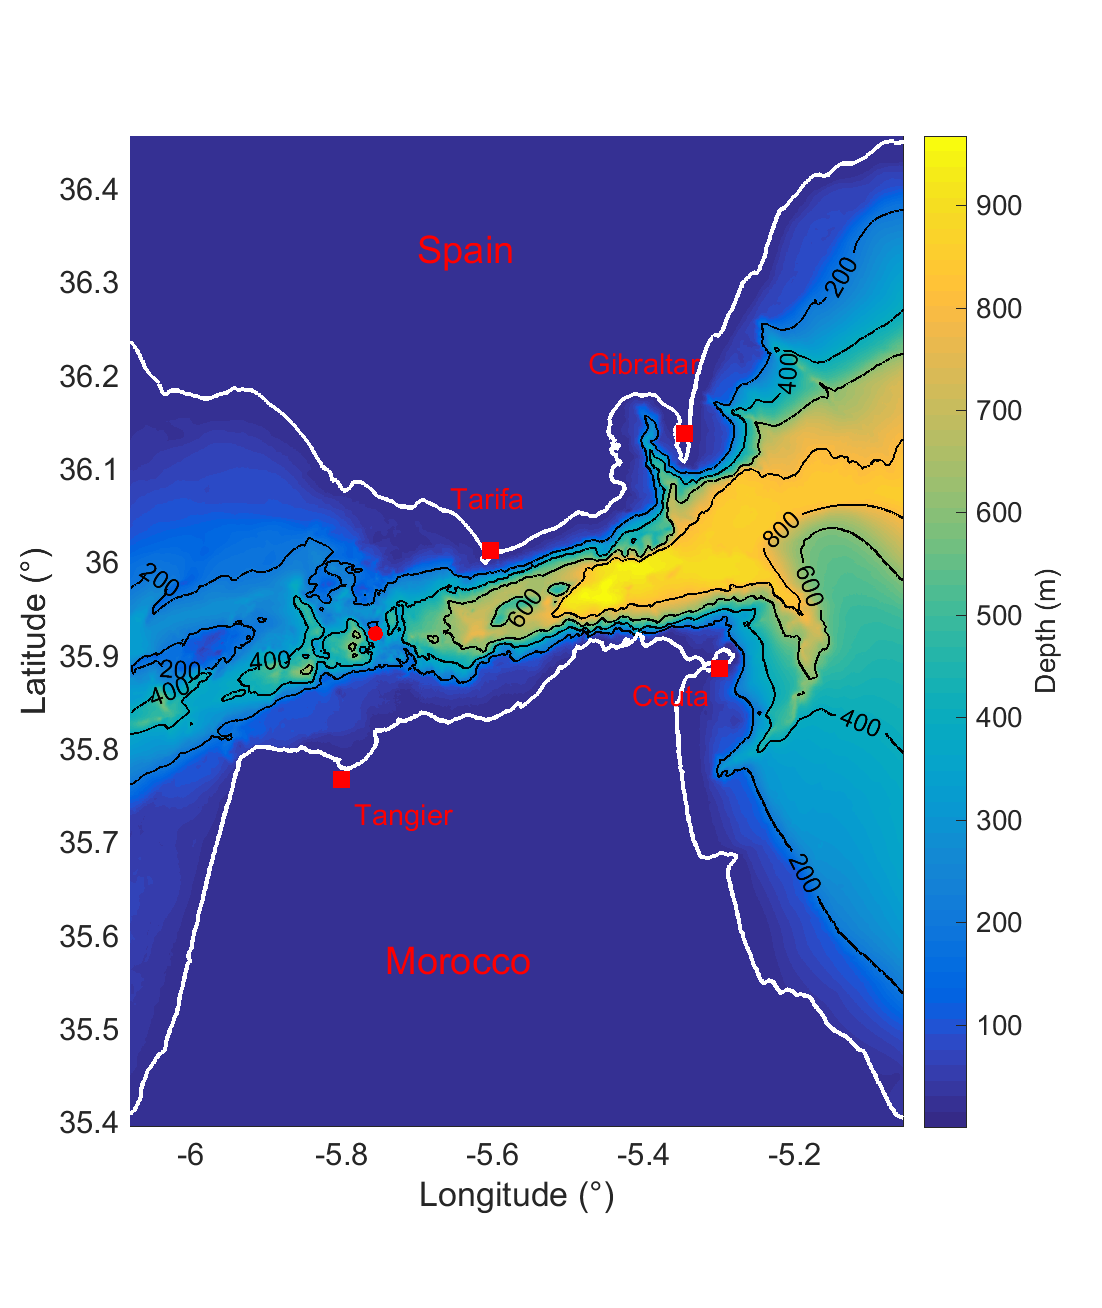
\includegraphics[width=0.5\textwidth]{./GBR3D/FigBathyVHR.png}
        \caption{Area and Bathymetry used for the simulations. The red dot denotes the point at Camarinal Sill where the zonal barotropic current is taken as reference in following figures.!!!Changer en anglais tangIer}
        \label{FigBathy3D}
\end{figure}



\begin{figure}[!h]
        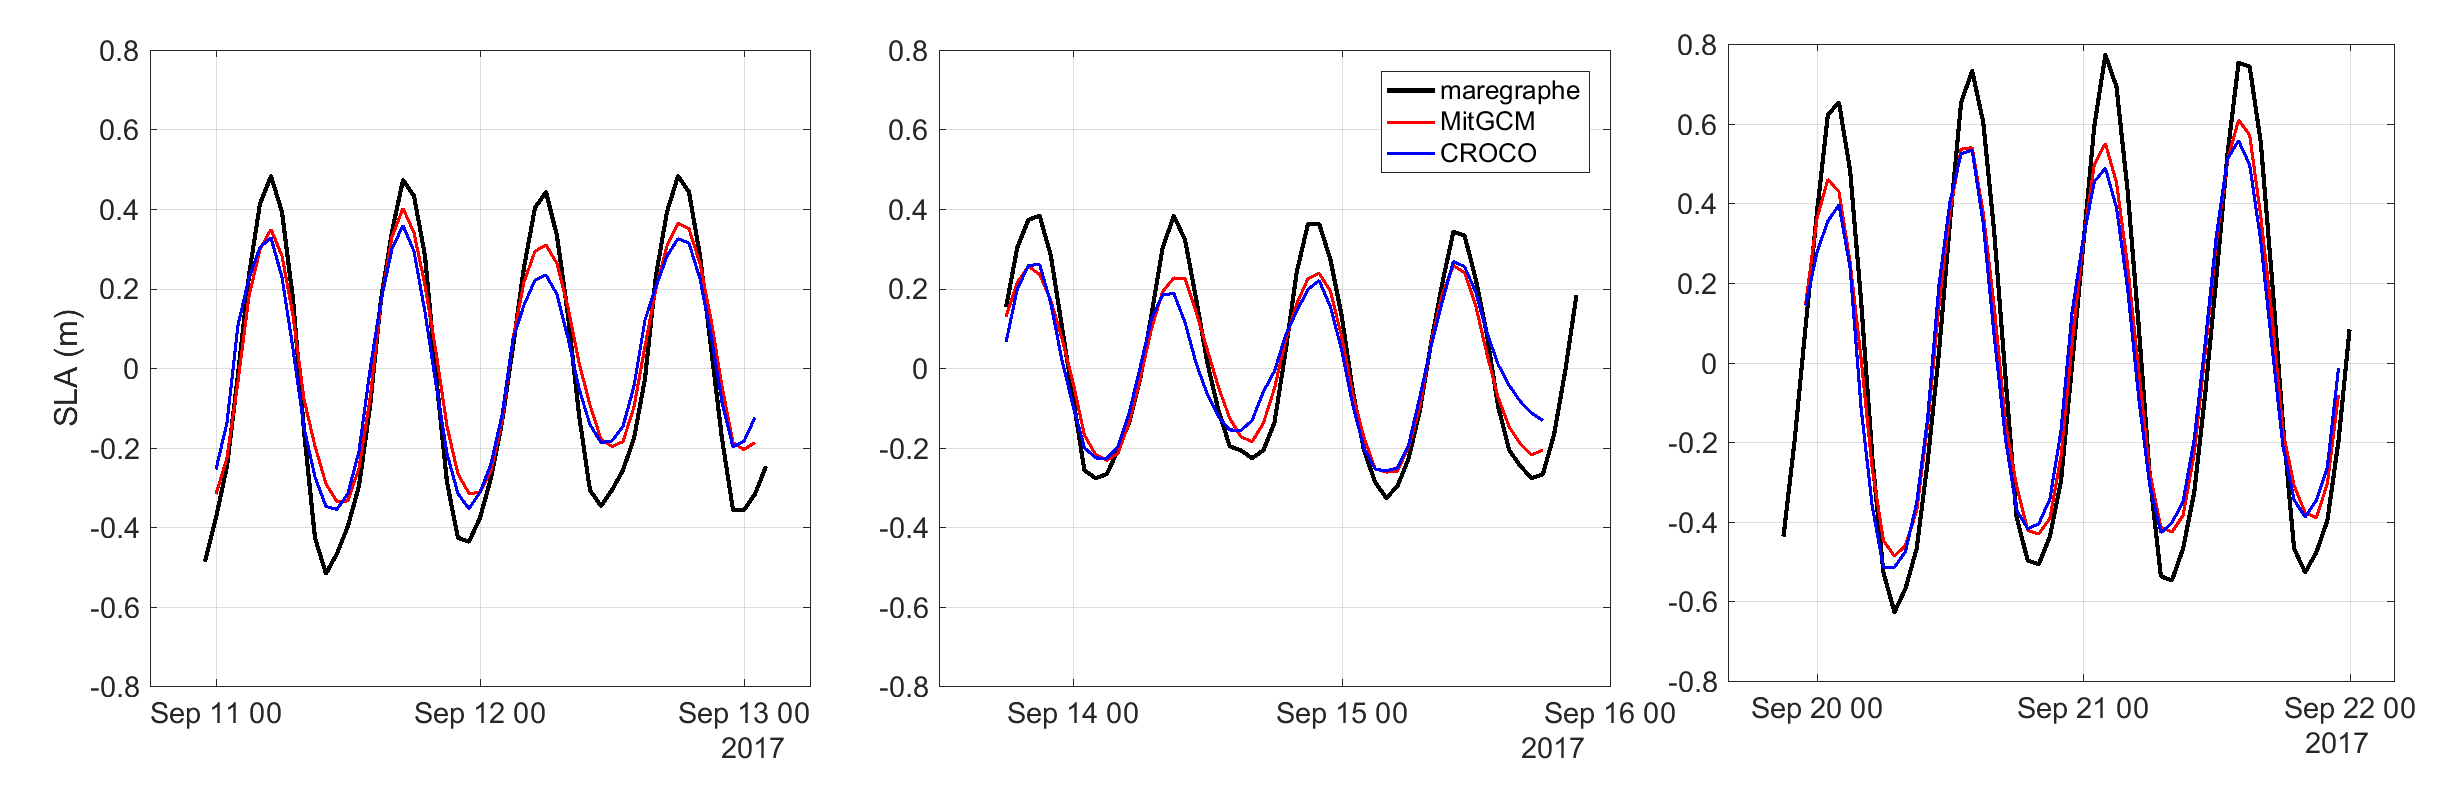
\includegraphics[width=\textwidth]{./GBR3D/SLA_Tarifa_ME2VE2IES.png}
        \caption{Sea level-anomaly at Tarifa from tidal gauge data (black) or at the nearest grid point for parent simulation (red) and CROCO simulation (blue), for situation ME (a), MM (b) et VE (c)}
        \label{fig_maree_tar}
\end{figure}

\subsubsection{Water masses}


\begin{figure}[!h]
        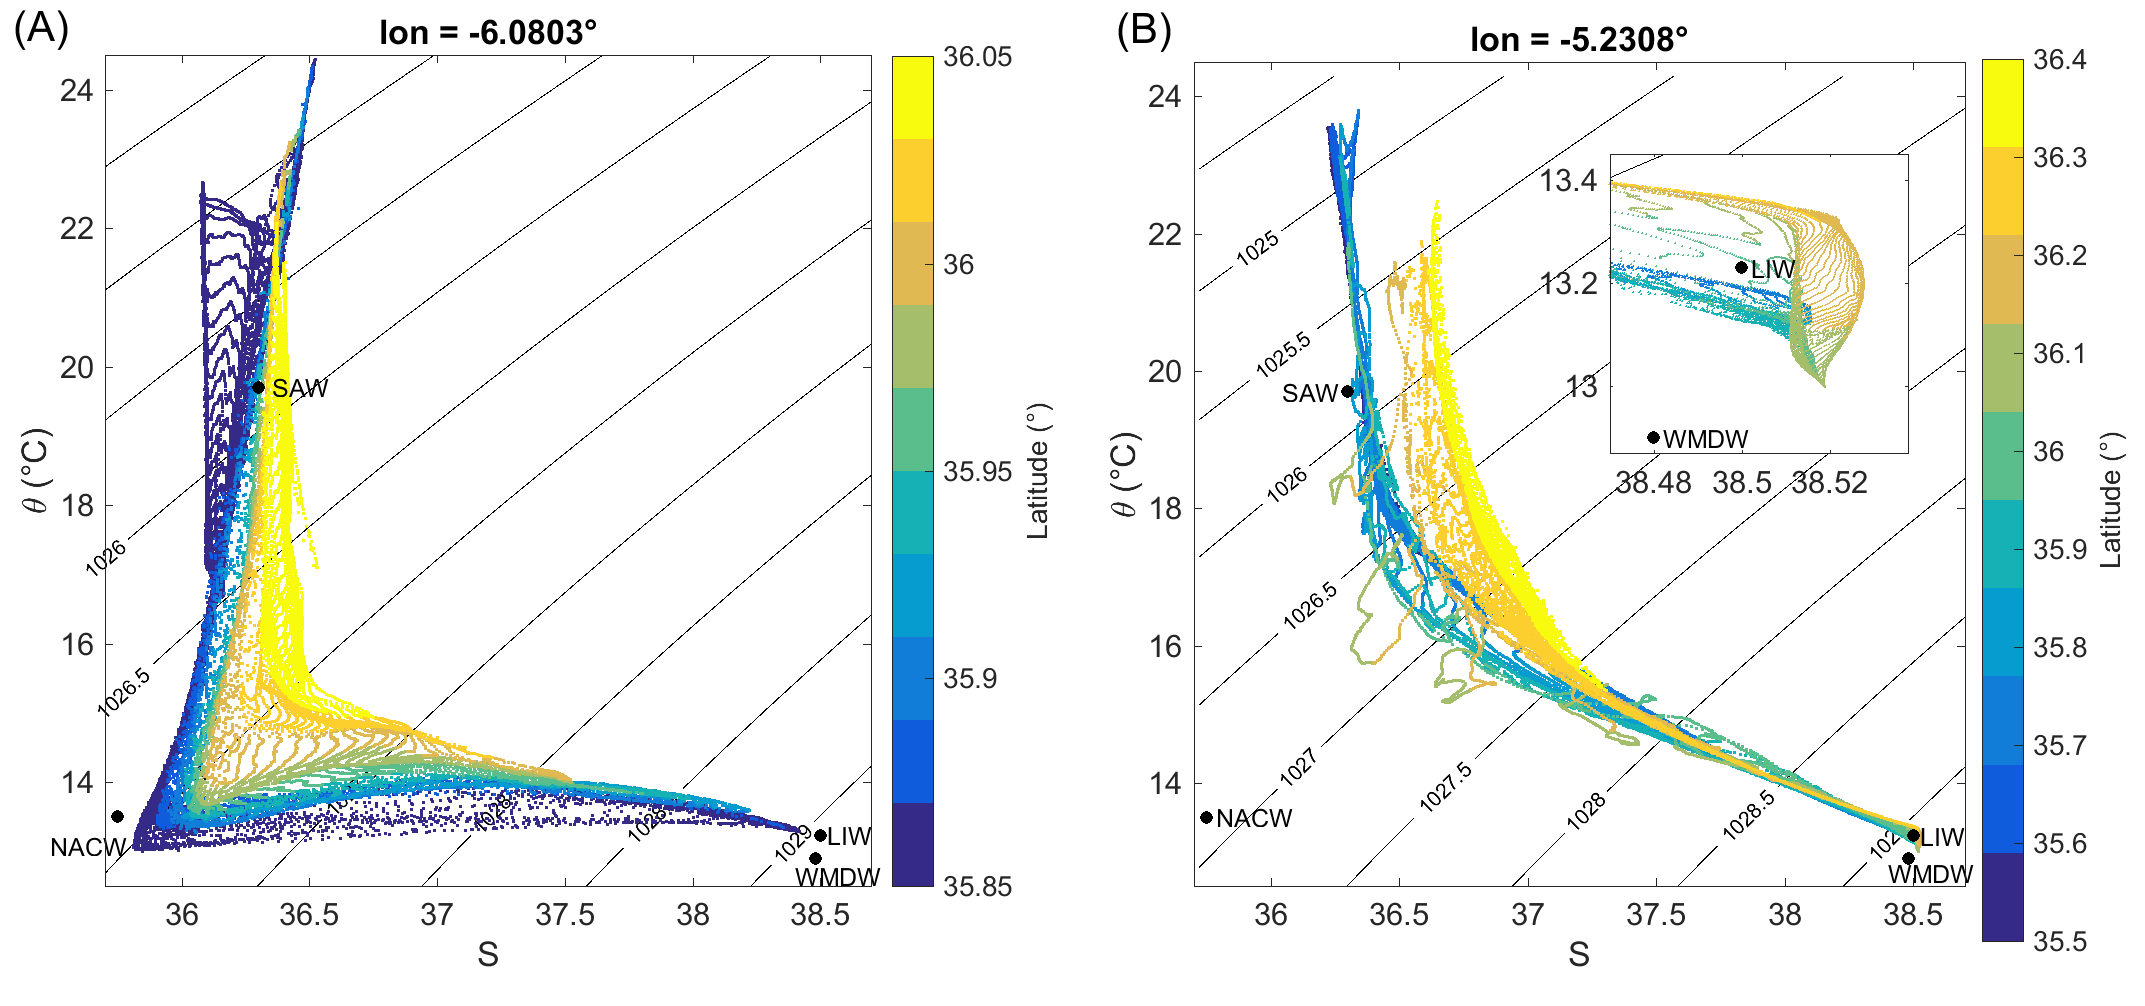
\includegraphics[width=\textwidth]{./GBR3D/WM_ini_IES.png}
        \caption{$\Theta$-S diagrams of grid points at 6.08$^\text{o}$W (a) and 5.23$^\text{o}$W in first timestep of SimIT, color indicates the latitude of each grid point. Are indicated cenroid definition of certain water masses according to Najanro2014}
        \label{Fig_Ini_WM3D}
\end{figure}


Figure \ref{Fig_Ini_WM3D} shows the $\theta$-S diagrams for east and west entry of the Strait in initial tracer field of simulation SimIT. As expected, for med waters see on the west side two signals for the two pathways of the med outflow, on the east side see distinctly a deep water mass and an intermediate one that could be interpreted as analogous to WMDW and LIW, with the latter being present mostly on the northern part, however in the simulation saltier and warmer waters than expected in bibliography. For atl waters, NACW present on west of domain, less on east. On east side, see difference surface water north/south of the opening of the Strait, with saltier surface waters in the north.




\subsection{Numerical diagnosis}
\label{PartDiag3D}

\subsubsection{Interface definition}

The analysis of simulation result is based on two layer definition of an Atlantic waters layer and Mediterranean waters layer. They are defined in regard to a reference salinity, with the interface defined as the height of the first water parcel from the top down in the water column for which salinity is above the reference salinity.

The reference salinity is taken as varying along the Strait as a hyperbolic tangent function of longitude centered at the Camarinal Sill to account for the different water mass composition in the eastern and western part of the Strait of Gibraltar. 

\begin{equation}
	S_i(x)=tanh(\frac{x-X_{CS}}{DX})\frac{S_M-S_m}{2}+\frac{S_M+S_m}{2}
\end{equation}
with $X_{CS}=5.75^o$, $dx=0.25^o$, the location and width of the Camarinal Sill in degrees, $S_M=37.39$ and $S_m=37.1$ the max and minimum values taken respectively east and west of the sill.

%This may not give the perfect interface at any given time...

\subsubsection{Froude layer number}

With the atlantic and mediterranean layers defined as above, the Froude layer number for internal gravity wave is computed at each 2D grid point as : 

\begin{equation}
F_i=\frac{U_i^2}{g'h_i} , \ \text{with} g'=g \frac{\rho_2-\rho_1}{\rho_0}
\end{equation}

where $\rho_i$ averaged density in layer i,  $U$ is averaged velocity norm over the layer i of height h. If $F_i>1$ say that the flow in layer i is supercritical.


\subsubsection{Hydraulic Jump detection, acceleration of flow}

\begin{figure}[!h]
 \centering
 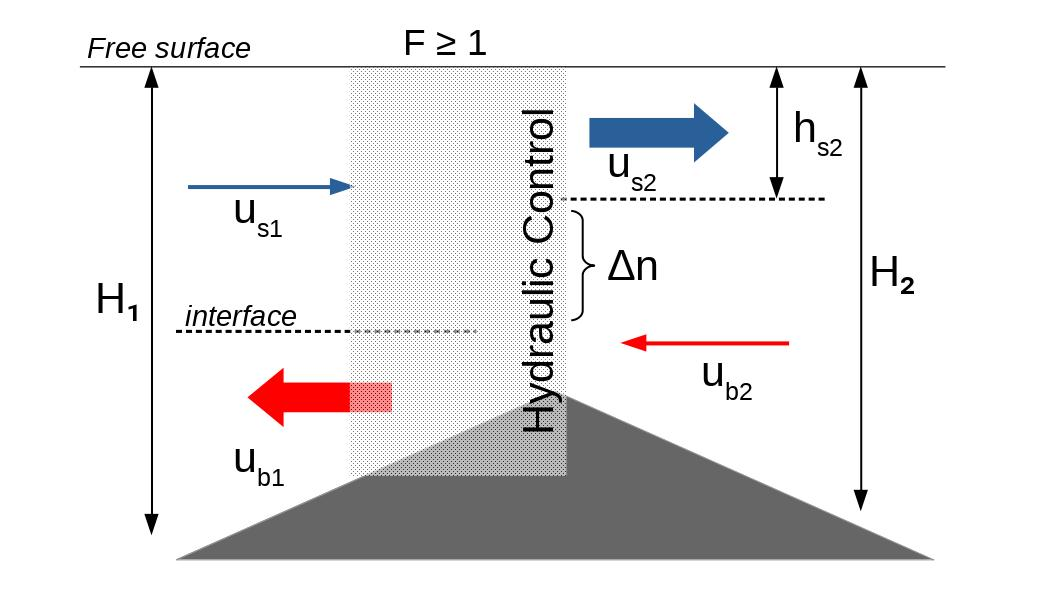
\includegraphics[width=0.5\textwidth]{./GBR3D/schema_diagressaut.jpg}
 \caption {Schematic of flow upstrean and downstream of hydraulic jump at Camarinal Sill, Strait of Gibraltar}
  \label{schemaRH}
\end{figure}


A simple diagnosis for detection of the hydraulic jump at Camarinal Sill in the simulations is based on the impact such a structure has on the flow. As shown/schematized/sketched(?) in figure \ref{schemaRH}, hydraulic jump (also called hydraulic drop) induces a drop of the interface depth. Since the flow in the Strait is canalised by bathymetry (for med flow) and coast (for atl flow), there must be conservation of flux from one section downflow and upflow of the hydraulic jump, which with the variation of the interface depth, means acceleration/deceleration of flow (depending on which layer is reference).

The drop in interface depth is noted $\Delta n=b_2-b_1$, the variation of bottom depth $\Delta H=H_2-H_1$ and the acceleration in the bottom layer $\Delta u_b = u_2-u_1$. For the bottom layer conservation of flux is :
\begin{subequations}
\begin{alignat}{2}
  \displaystyle
&u_1 (H_1-b_1)&& = u_2 (H_2-b_2)\\
& &&= u_1 (\Delta H + \Delta n) + u_1 (H_1-b_1) + \Delta u_b (H_2-b_2)
\end{alignat}
\end{subequations}

\begin{equation}
\Delta u_b = -u_1 \frac{\Delta H + \Delta n}{H_2-b_2}
\end{equation}

For the surface flow, similarly can find
\begin{equation}
\Delta u_s = - u_1\frac{\Delta n}{b_2}
\end{equation}

Velocity in the area of the hydraulic jump must validate condition of (at least) critical flow, ie Froude number $\geq$ 1. We search minimal condition for hydraulic jump so $F=1$, or $U=c$, taht is the flow ceerity equals the phase speed of internal wave. If for the latter we take the definition of interfacial speed can have an expression for $u_1$: 
\begin{equation}
|u_1|=c=\sqrt{g' \frac{(H_1-\Delta n - b_2)(\Delta n + b_2)}{H_1}}
\end{equation}



In the end, some parameters are chosen as threshold, here take values that should be correct for area of camarinal sill, the minimum excursion of the jump $\Delta n = 30m$ and the height of the Atl layer $b_2=50 m$ , and the reduced gravity $g'=0.02 m s^{-2}$.

\subsubsection{Q parameter and derivated diagnosis}

We want to detect primary shear instabilities in the Med outflow. A simple vorticity diagnosis is not chosen as it requires choosing the rotation axis, but also because regions of high shear such as between the MEd outflow and Atl waters will have high vorticity values. Instead, analogously to the use of the Okubo-Weiss parameter in Hilt 2020, we chose to compute parameter Q, defined as (ref):

\begin{equation}
Q=-\frac{1}{2} \frac{\partial u_i}{\partial x_j} \frac{\partial u_j}{\partial x_i} = \frac{1}{2} (\Omega_{ij}\Omega_{ij} - S_{ij} S_{ij})
\end{equation}
with $u_i$ the components of velocity vector, and $S_{ij}$ and $\Omega_{ij}$ are respectively the strain-rate tensor and vorticity tensor. When $Q>0$, rotation is predominant over shear part.


Due to advection by the Med outflow, a succession of primary instabilities will propagate over teh same grid cells. The temporal evolution of Q over such grid cell will show oscillations between high positive value (center of a billow/vortex) and low negative values (shear between two consecutive billows). A proxy to detect this area is chosen as high value of standard deviation of parameter Q, as defined in equation \ref{eqstdQ} where the over bar denotes temporal average over 30 minutes, a period over which there will be minimal modification of the general flow in the Strait.

\begin{equation} 
\label{eqstdQ} 
    std ( Q ) (\vec{x},t)=  \sqrt{   \overline{Q (\vec{x},t)^{2}} -  \overline{Q(\vec{x},t)}^{2}  }
\end{equation}

To create 2D maps presented in next section, only the maximal value of standard deviation in the water column is saved...
By implementing this calculation directly in the code, we can asses where instabilities/vortexes propagate without having to make a huge volume of simulation outputs over the whole domain, those economising in storage place and data readability. 

The result of this proxy can be compared to the result of the Singular Value Decomposition (SVD) of the time-varying 3D field. However this calculation is off-line and necessitates a high frequency 3D output to pick up the relevant structures.



\subsection{Results}
\label{section3DRes}

\subsubsection{Flow criticality/Hydraulically controlled layer and hydraulic jump, neap-spring tide variability}


\begin{figure}[!h]
 \centering
 
 \begin{subfigure}{\linewidth}
\centering
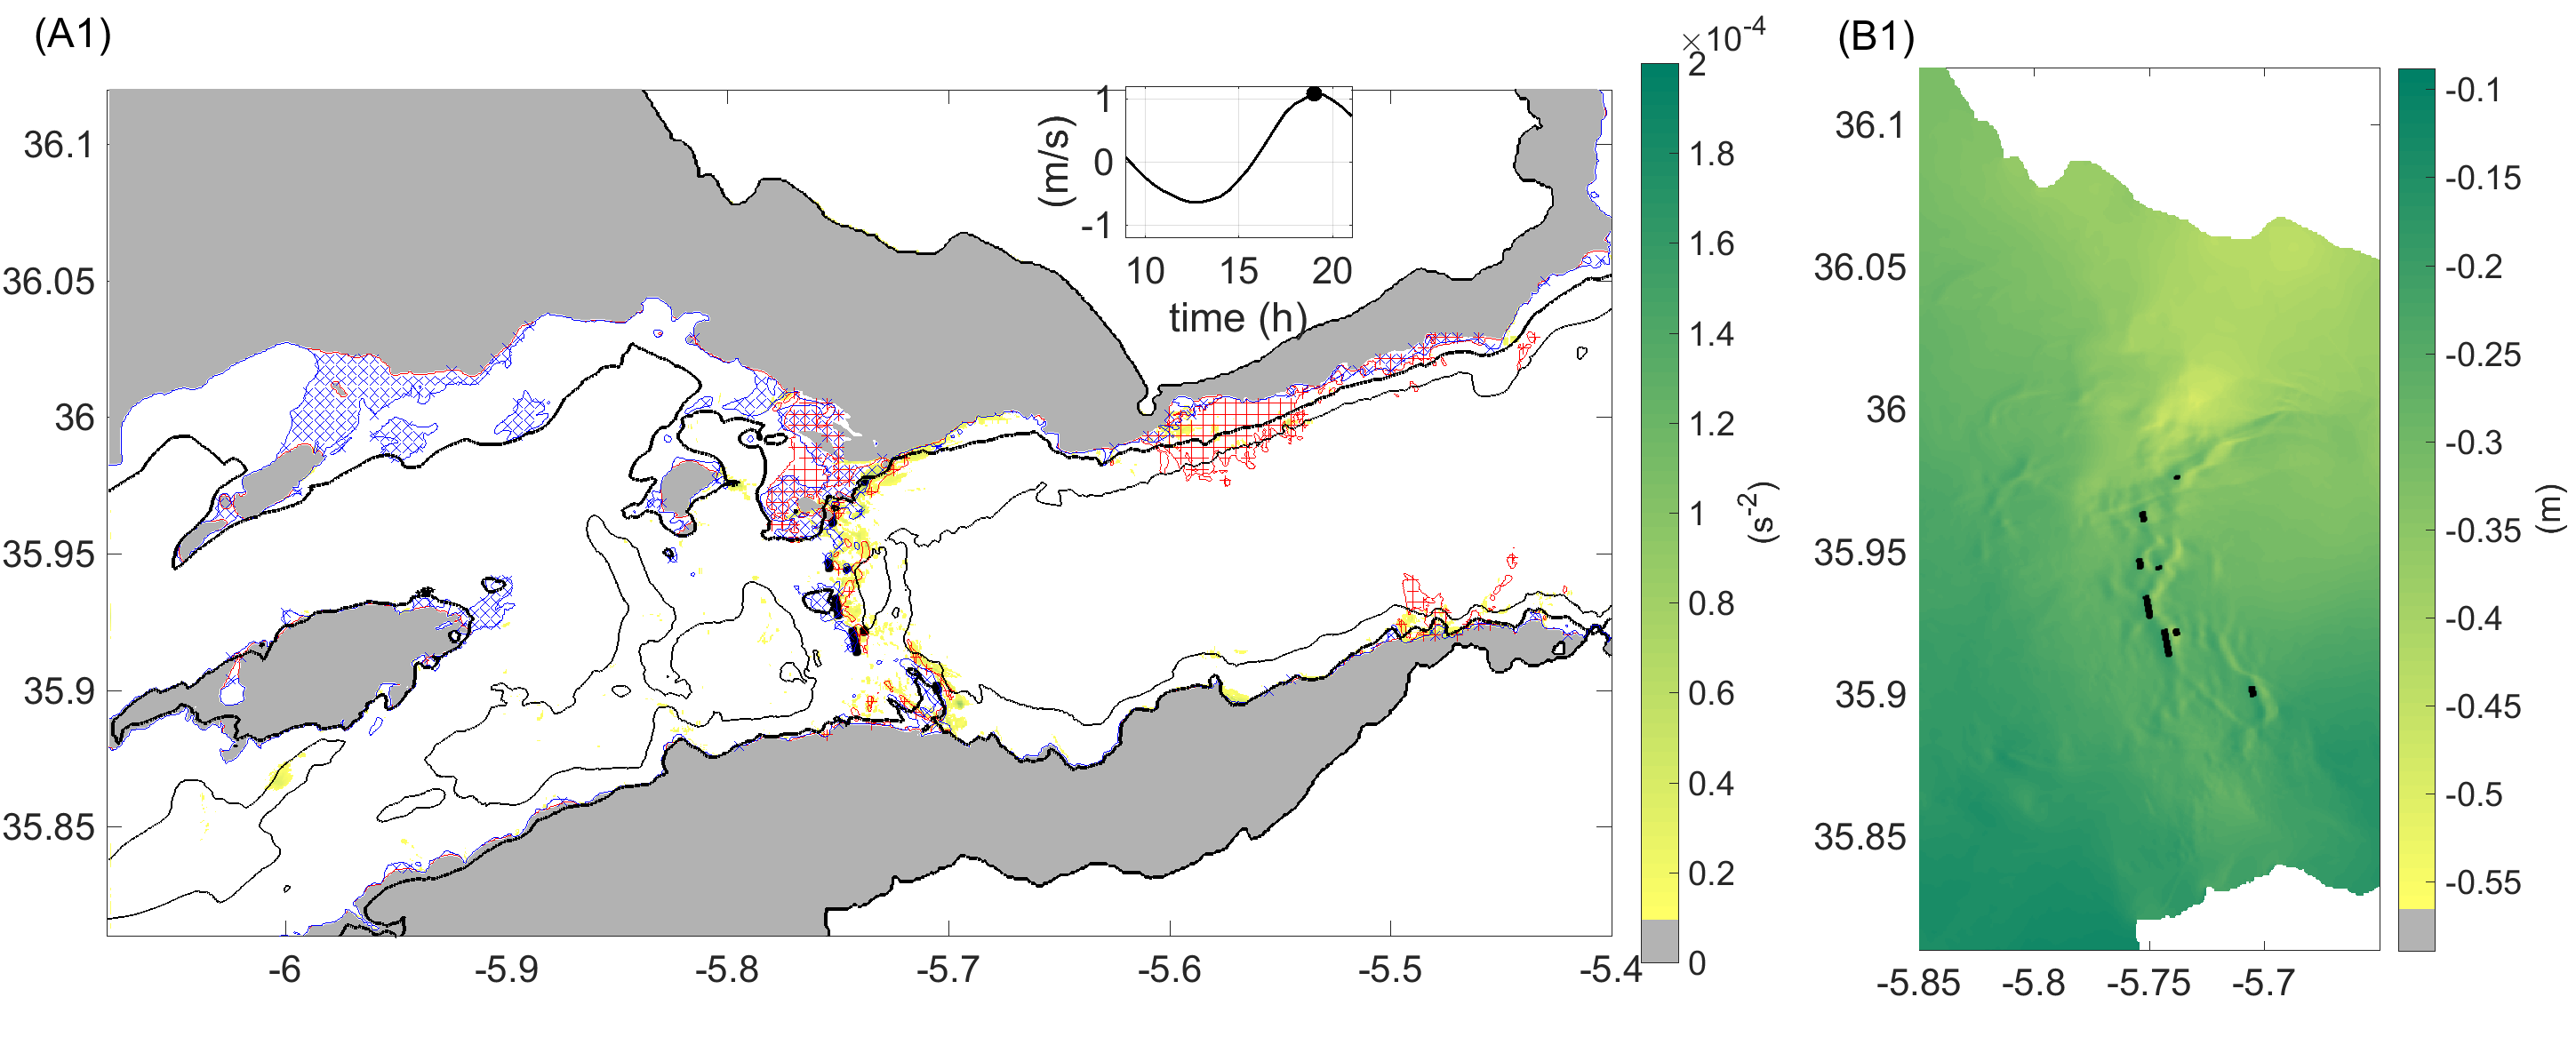
\includegraphics[width=1\linewidth]{./GBR3D/ME2_19h_p.png}
\end{subfigure}
 
 \begin{subfigure}{\linewidth}
\centering
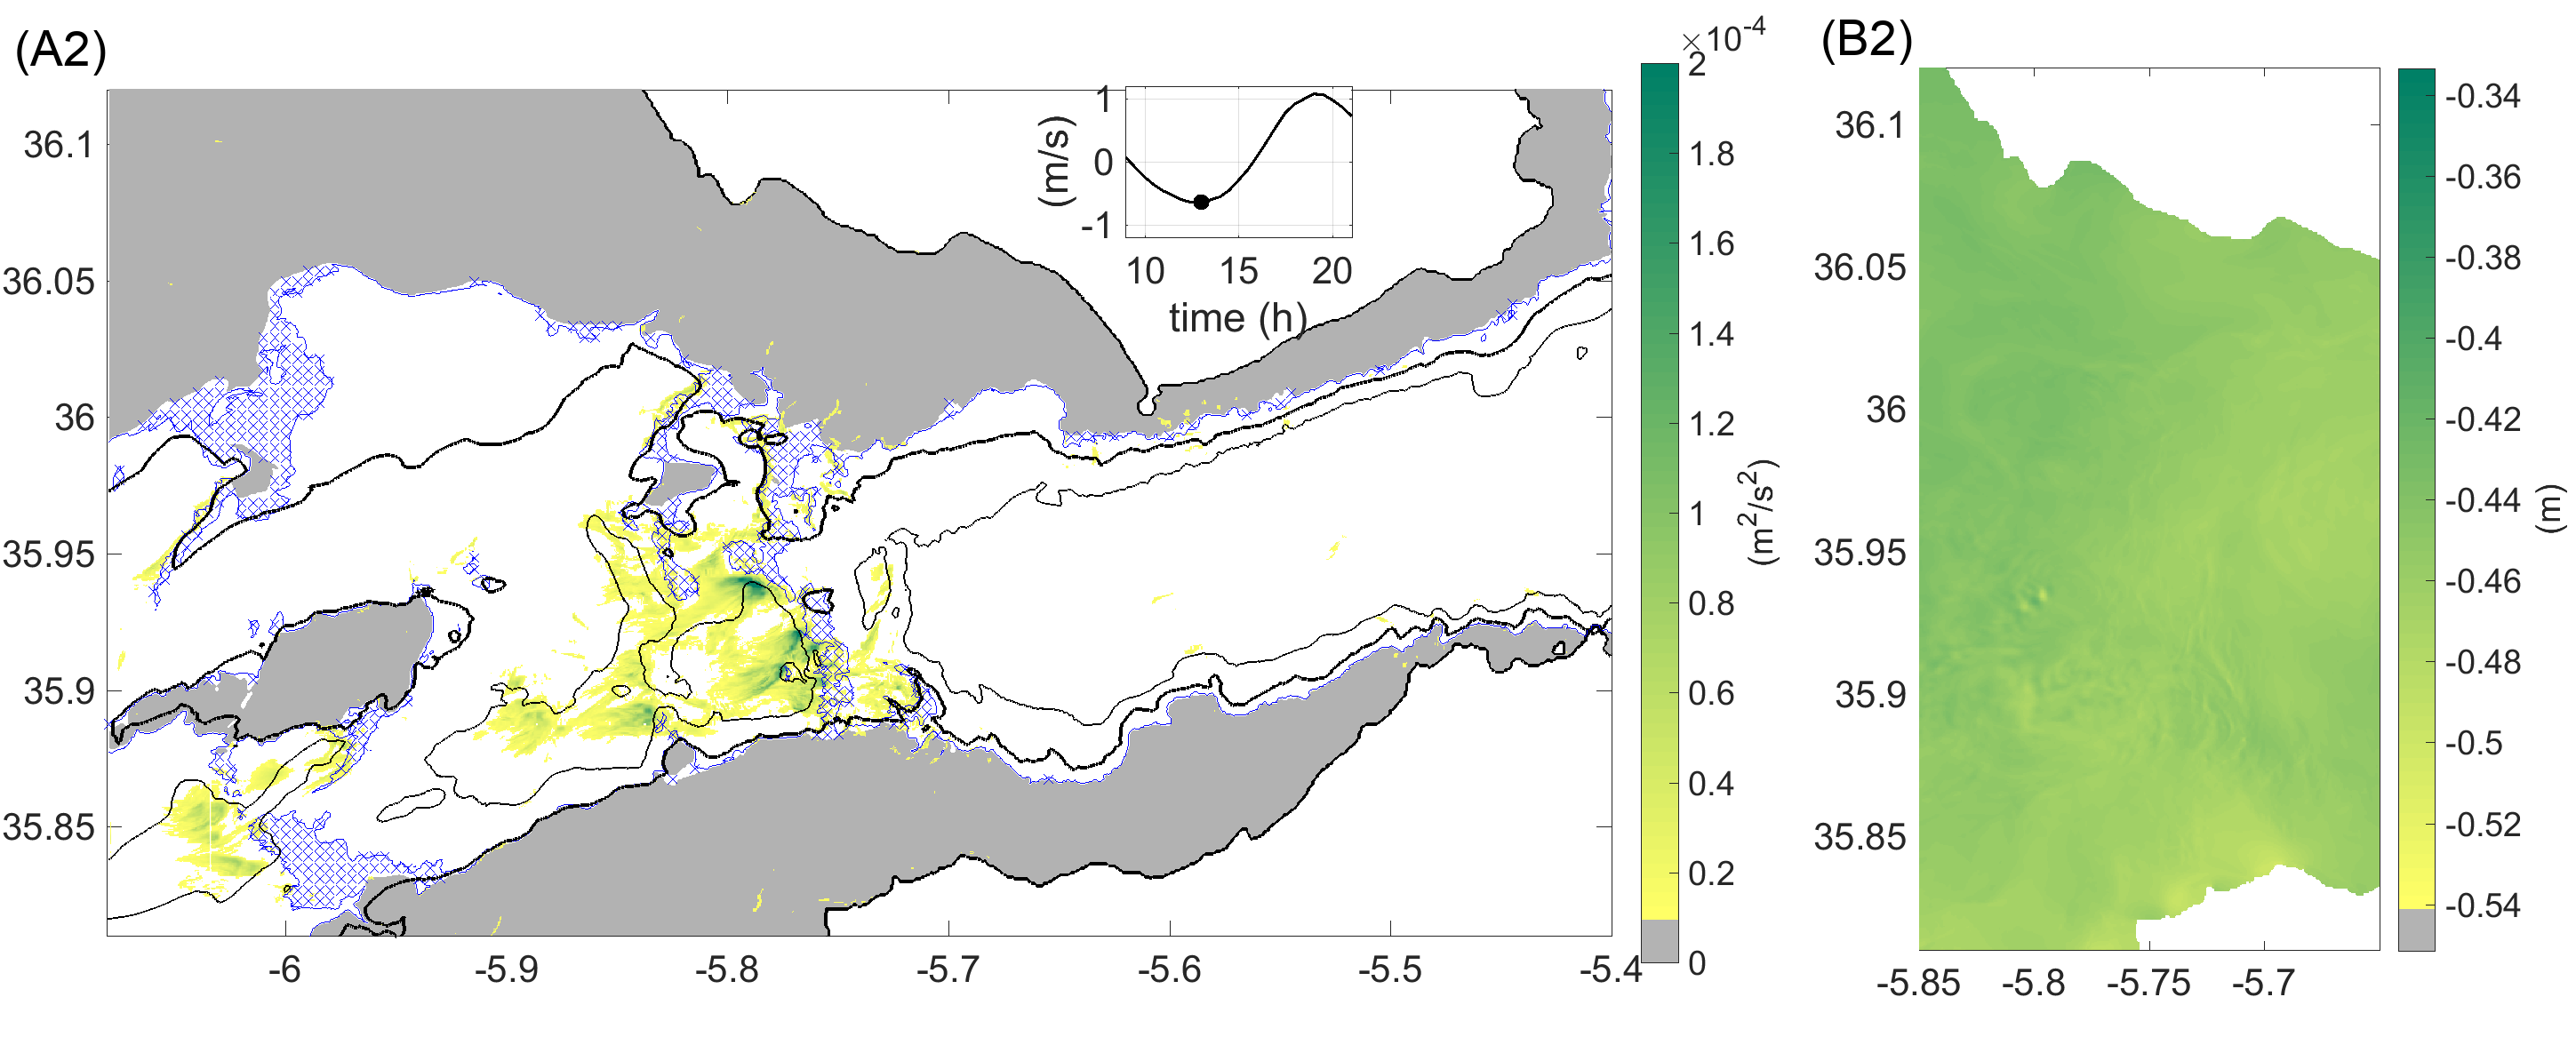
\includegraphics[width=\linewidth]{./GBR3D/ME2_13h_p.png}
\end{subfigure}
\caption {For simulation SimNT, an inflow then an outflow of type \textit{no-jump}. Blue (red) shaded area is supercritical med (atl) layer. Black dots are hyd jump detection. grey area denotes where S bottom$<$Sinterface. colorbar for standard deviation of parameter Q (only values above $10^-5$are represented). Also inicated barotropic znal current at CS (point indicated in figure \ref{FigBathy3D}). Two black isobathes contours are indicated, 200m (bold) and 400m(thin) depth  }
\label{FigHCN}
\end{figure}

Figures \ref{FigHCN} to \ref{FigHCI} present several diagnosis for series of maximal outflows and inflows for variable strength of the tidal forcing among simulations SimNT,SimST then SimIT. Are represented the diagnosis presented in paragraph \ref{PartDiag3D} : the area of supercritical flow in atl and med layer as shaded areas, the detection of hydraulic jump, and area of standard deviation of parameter Q, which indicate were vortices are propagating. The grey area indicates where the salinity in the bottom level is below the interfacial salinity as defined in paragraph ..., and thus were it is considered only Atlantic waters circulate.

Figure \ref{FigHCN} presents a situation of weak barotropic currents ($<1m/s$ at a shallow point of Camarinal Sill) in outflow and inflow and is considered a 'neap-tide' case, figure \ref{FigHCS} is for strong barotropic currents ($\geq 1.5m/s$) for the in- and outflow of a 'spring-tide' case. Finally, figure \ref{FigHCI} is the case of an outflow for an intermediate strength ($\approx 1m/s$)of the barotropic currents.

\begin{figure}[!h]
 \centering
\begin{subfigure}{\linewidth}
\centering
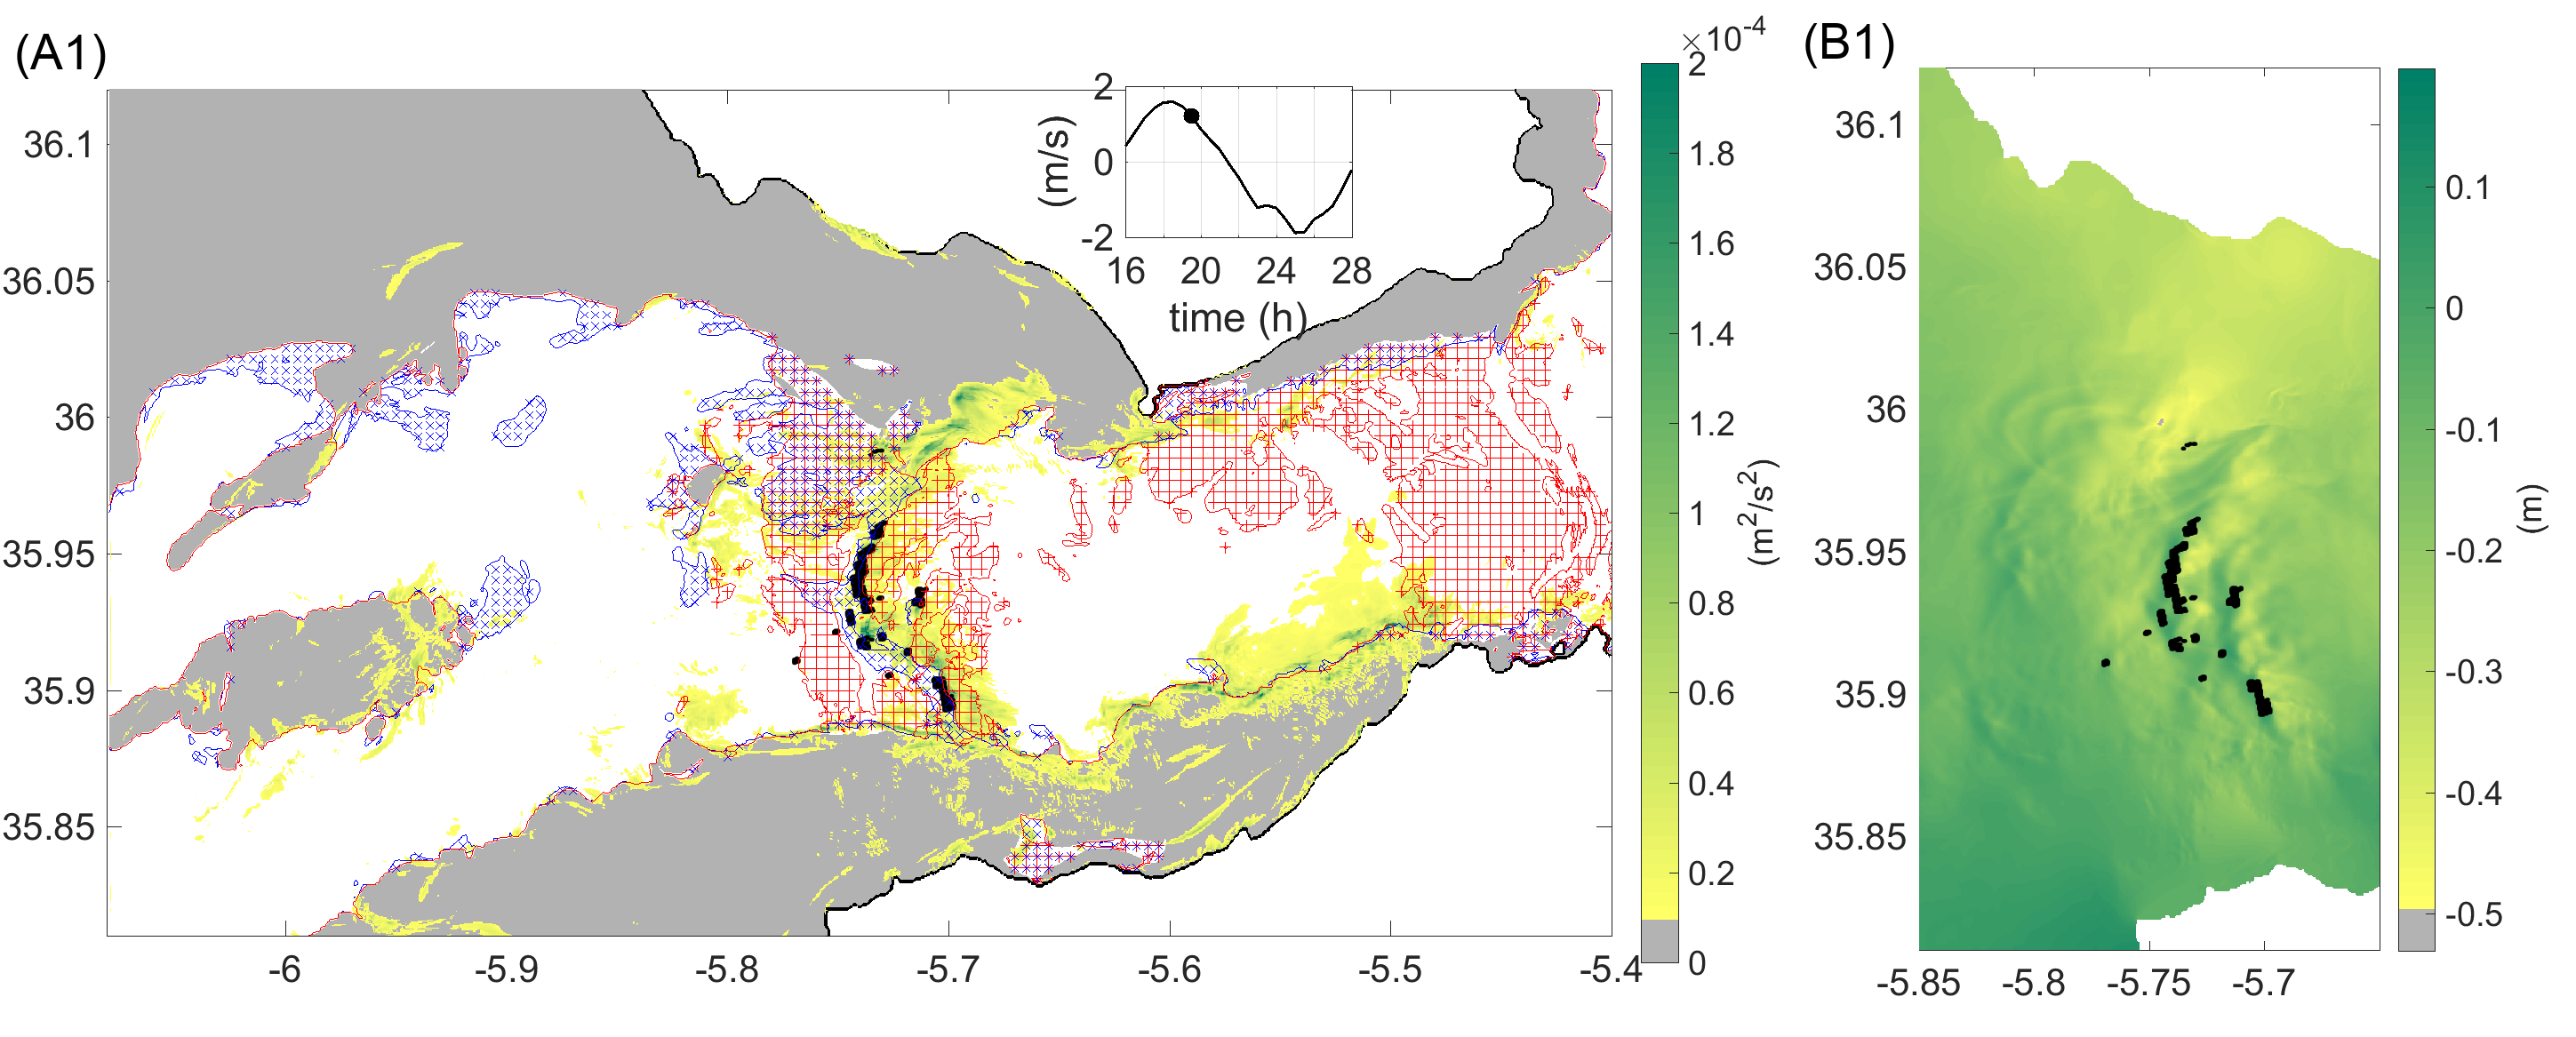
\includegraphics[width=\linewidth]{./GBR3D/VE2_19h30_p.png}
\end{subfigure}

\begin{subfigure}{\linewidth}
\centering
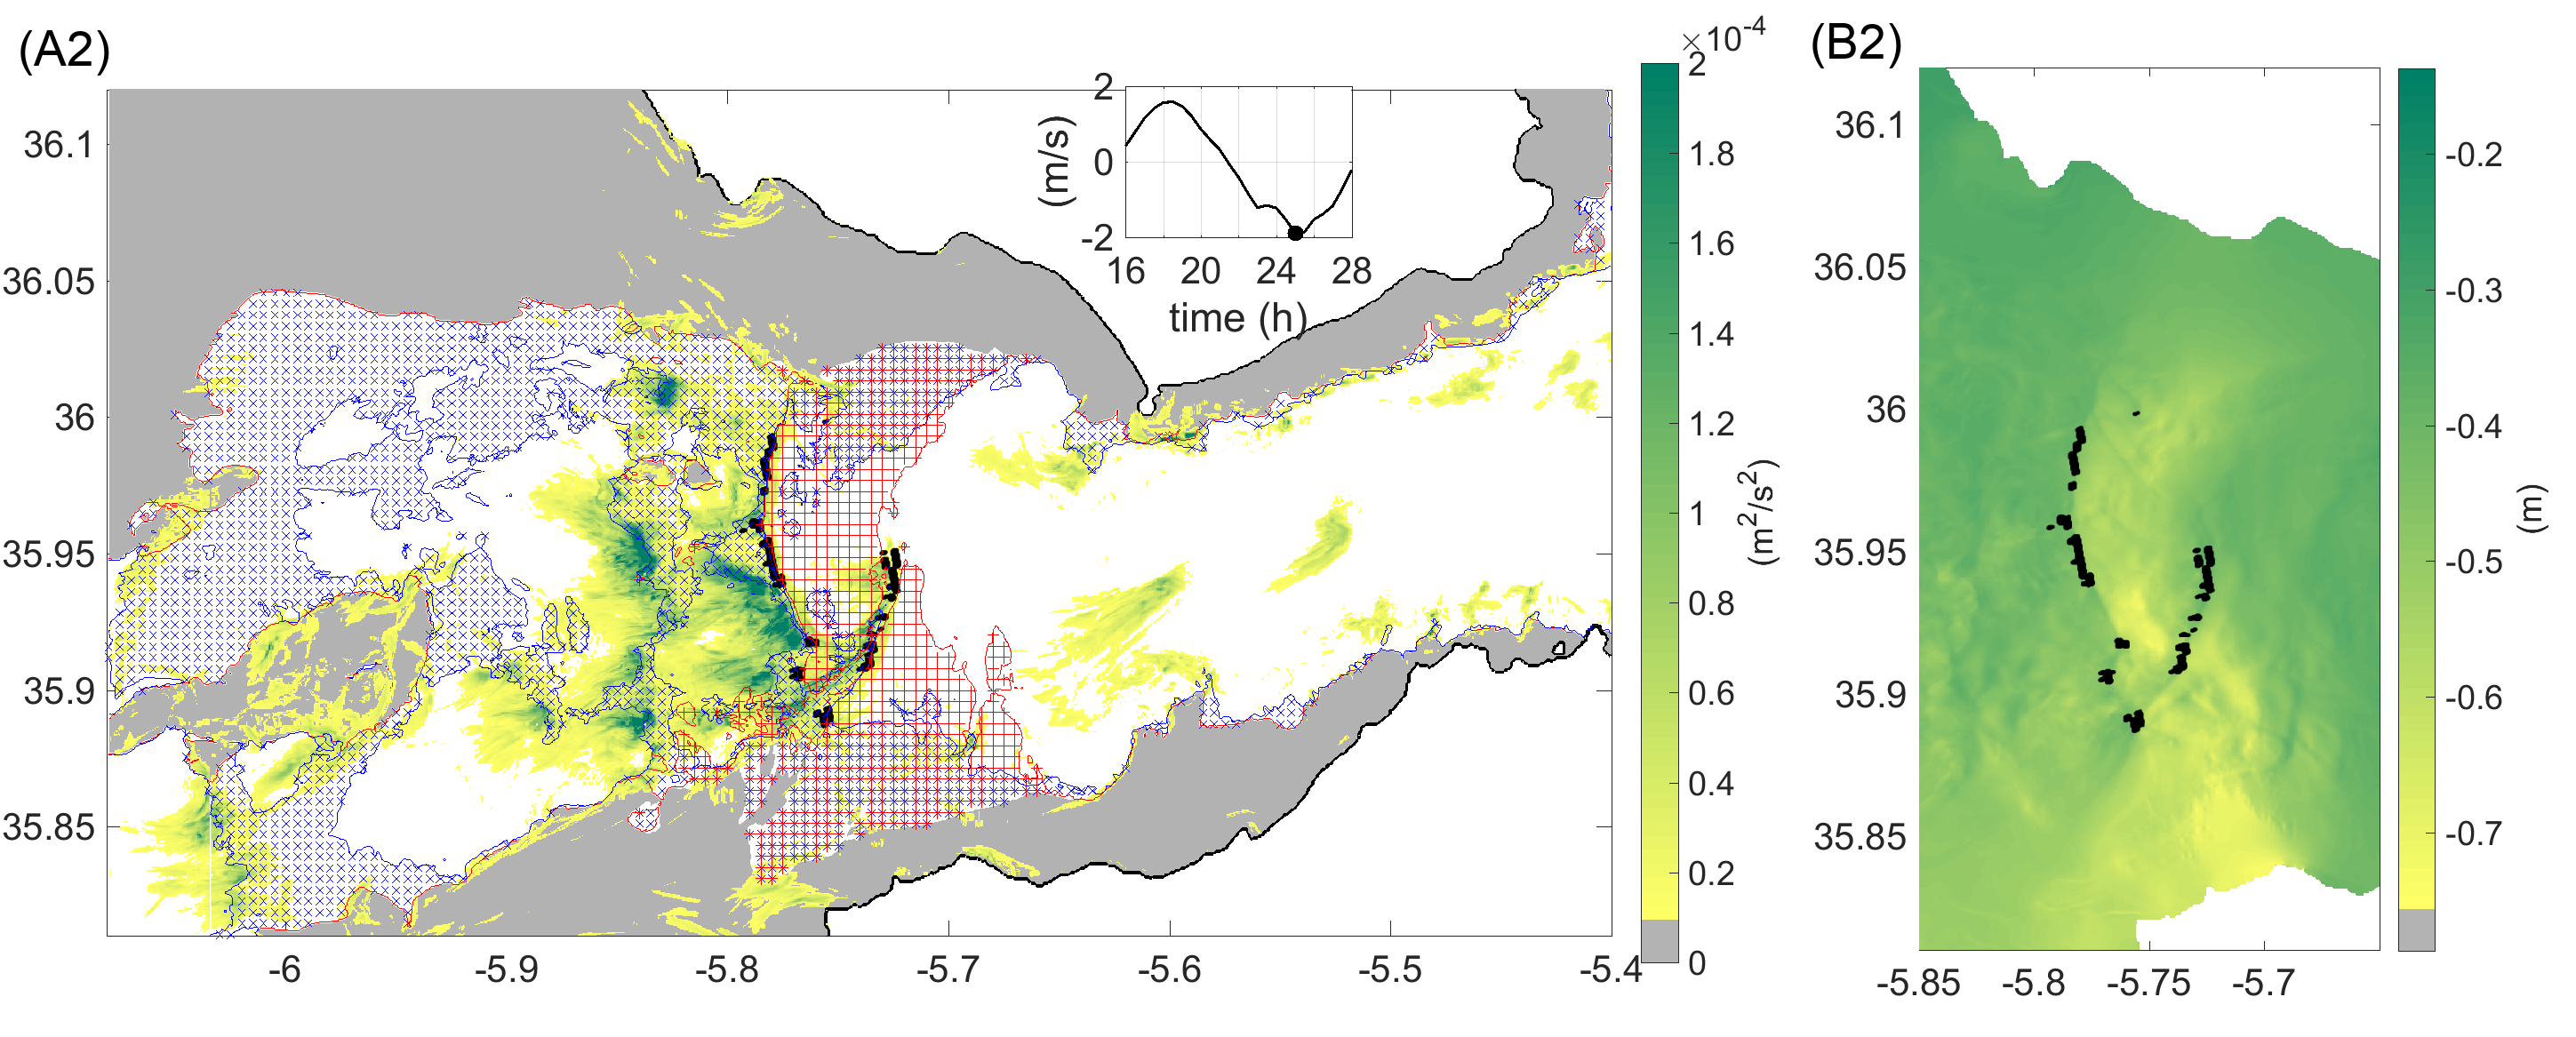
\includegraphics[width=\linewidth]{./GBR3D/VE2_25h_p.png}
\end{subfigure}
\caption {Same as figure \ref{FigHCN} for simulation SimST in inflow and outflow of type \textit{w-jump}}
\label{FigHCS}
\end{figure}

\begin{figure}[!h]
 \centering
%\begin{subfigure}{\linewidth}
%\centering
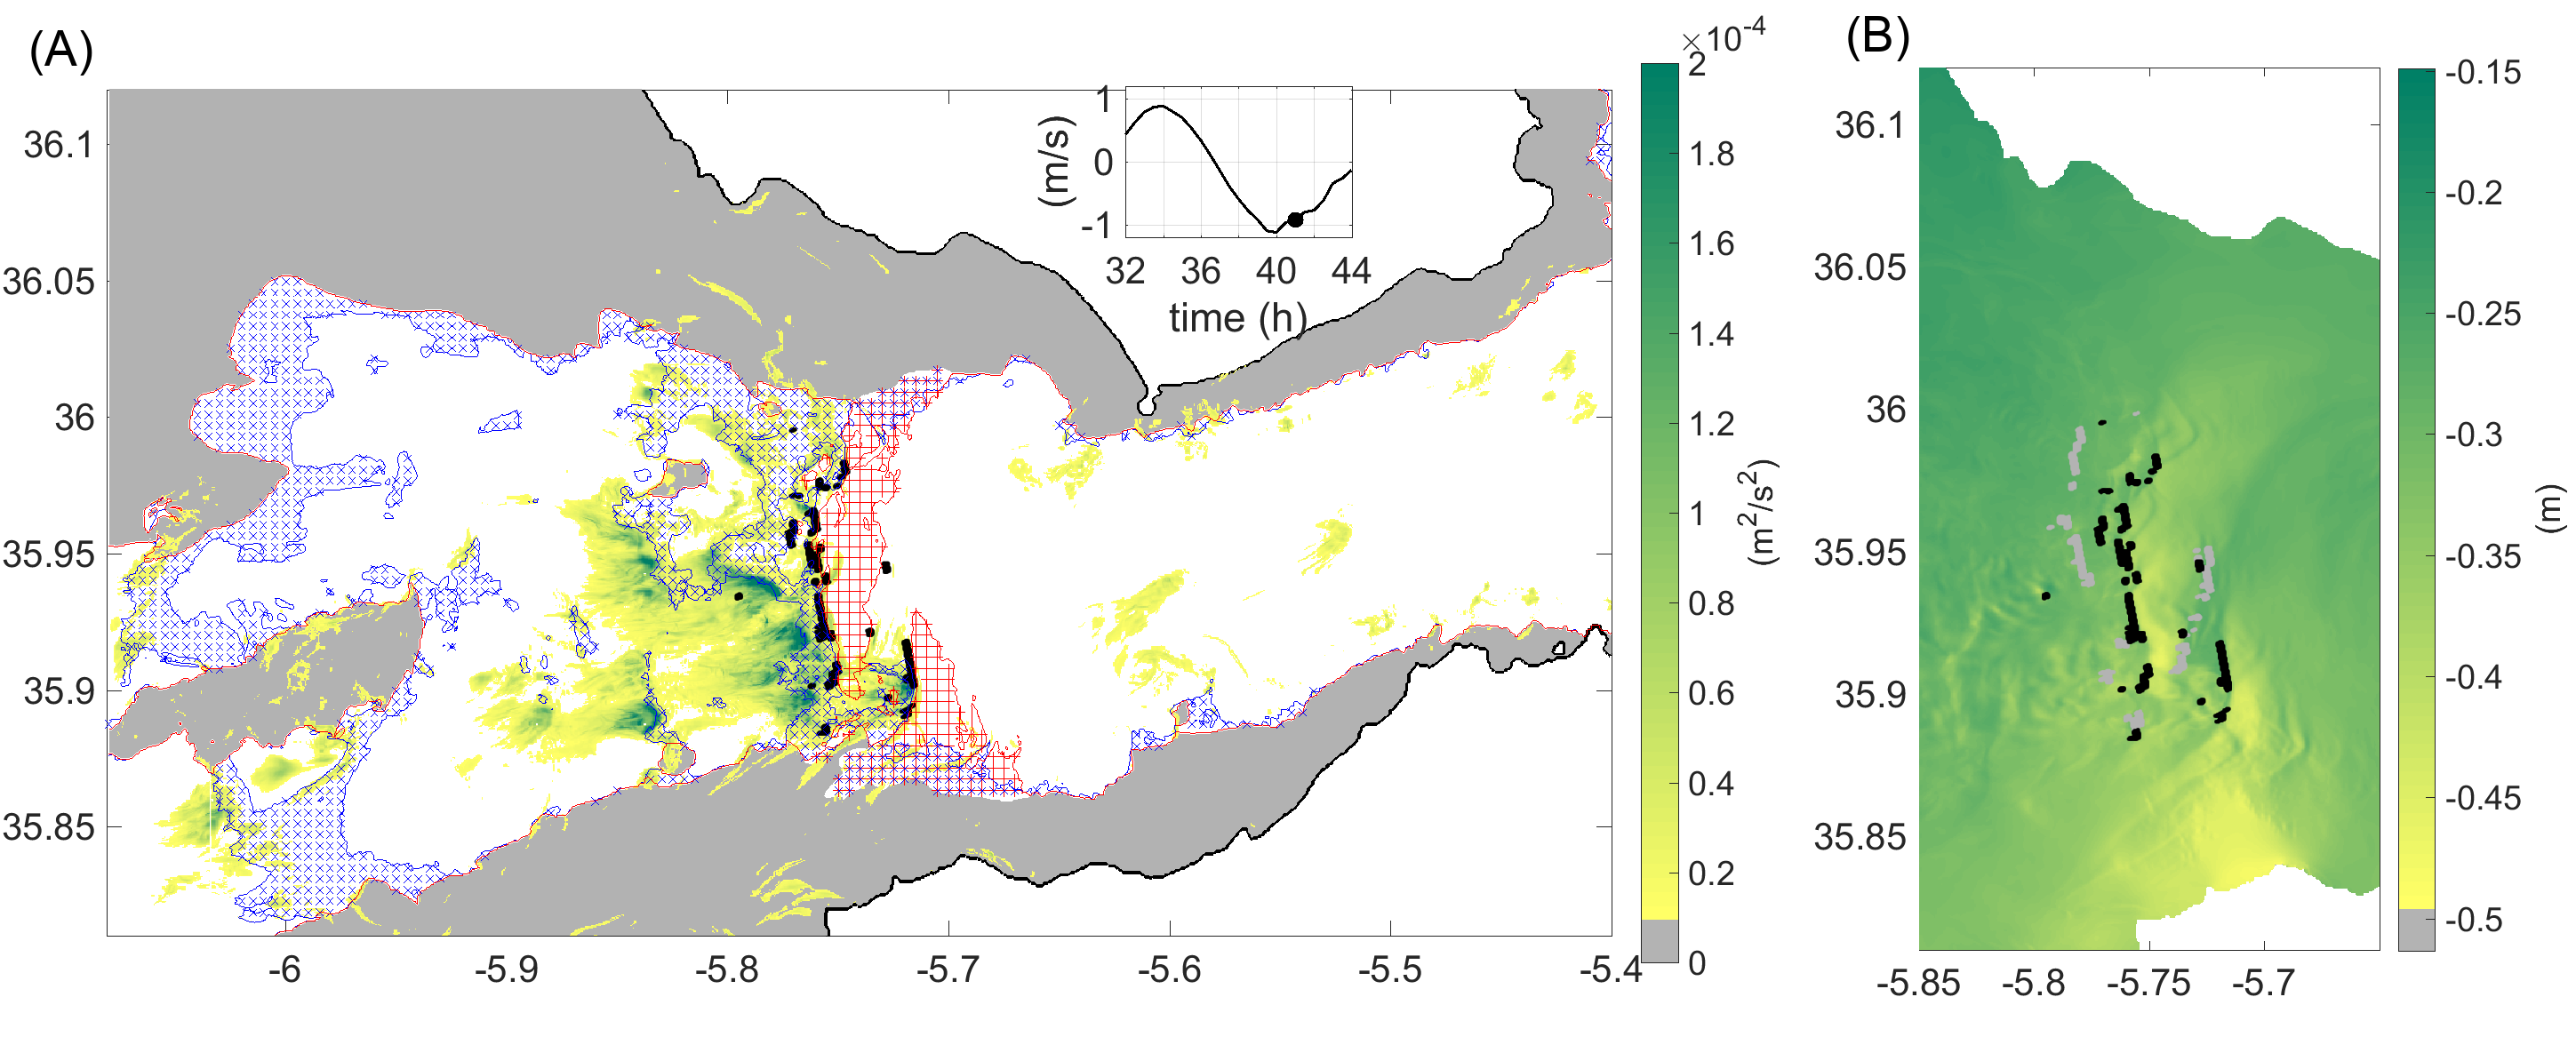
\includegraphics[width=\linewidth]{./GBR3D/IES_41h_p.png}
%\end{subfigure}
 \caption {Same as figure  \ref{FigHCN} for simulation SimIT and an outflow of type {s-jump}, on figure SLA also put trace of jump of spring tide outflow}
 \label{FigHCI}
\end{figure}

Firstly, can see two channels west of the Camarinal Sill where Med layer is present, separated by Majuan Bank. The path of the med vein through the south channel does not change much, however in the northern channel see a variable area of circulation for med waters above 200m depth and centered at 36$^\text{o}$ N. This area is larger during outflows, as med waters are driven up-slope by the westward barotropic current, but there is also a southern component to the flow that bends back into the main north channel (see figure \ref{FigBathy3D} for a better view of the bathymetry of the area).

For all cases, supercriticality of the atlantic (mediterranean) layer happens mostly east (west) of 5.8$^\text{o}$W which is the western slope of Camarinal sill. During inflows in figure \ref{FigHCN}.a and \ref{FigHCS}.a, criticality of the mediterranean layer only occurs in patches, the most extended one in the area of the northern channel discussed above. In outflows in figures \ref{FigHCN}.b,\ref{FigHCS}.b and \ref{FigHCI} the Mediterranean layer is supercritical at both Camarinal, Espartel Sill and northern channel for all cases. In the spring tide outflow case especially, most of the northern channel has a supercritical flow while at Espartel there is not much difference between the intermediate and spring tide outflow cases.


During outflow supercritical atl layer only at CS, except in neap case where it does not occur at all. In the case where both layers are supercritical at CS, hydraulic jump is detected. It is located at the junction between an area where atl and med layer are supercritical. It follows area of high gradient of free surface elevation.  Find accross all simulated tidal cycle three type of flow at Camarinal Sill during outflow : no hydraulic jump as in figure \ref{FigHCN}.b (\textit{no-jump}), a hydraulic jump situated just above the sill (figure \ref{FigHCI}, \textit{s-jump}), and a hydraulic jump situated over the west slope of the Camarinal Sill (figure \ref{FigHCS}.b, \textit{w-jump}). In this latter case, the hydraulic jump actually starts forming over the sill's crest as in the s-jump case but as the tidal currents strengthen, the area of supercritical atl layer area develops westward and so does the junction where can observe the jump.

Also see hydraulic jump during inflows, located in the same area over the east slope of CS regardless of the strength of tidal currents, but more pronounced with stronger barotropic currents, associated with transition of flow upstream of area of supercritical atl layer.

East of Camarinal Sill, another area of supercritical Atl layer appears during inflows. In neap-tide case, as a patch near north shore in TN at 5.59$^o$W. for spring tide case, this patch is more extended, and a secondary area of supercritical atl flow exists between 5.5$^o$W and 5.4$^o$W, extending from the north to the south side of TN. 

Figure \ref{FigISWGBR3D} shows the field of surface current divergence in Tarifa Narrows while a train of ISW is propagating, figure a for condition of intermediate strength of barotropic current in inflow and figure b for a strong barotropic current at the same time as figure \ref{FigHCS}.b. Are also shown the areas of critical atlantic layer flow as black meshed area. The propagation of the ISW train occurs at the same time as maximum inflow in this area and see the area of atl layer criticality is west of the propagating wave train . It seems the northern part of the criticality of the atl layer is dissociated from its southern part. The former occurs most often and is more or less extended while the other may be affected by influence of the passage of the ISW, either due to induced velocity or change of stratification.



\begin{figure}[!h]
 \centering
%\begin{subfigure}{\linewidth}
%\centering
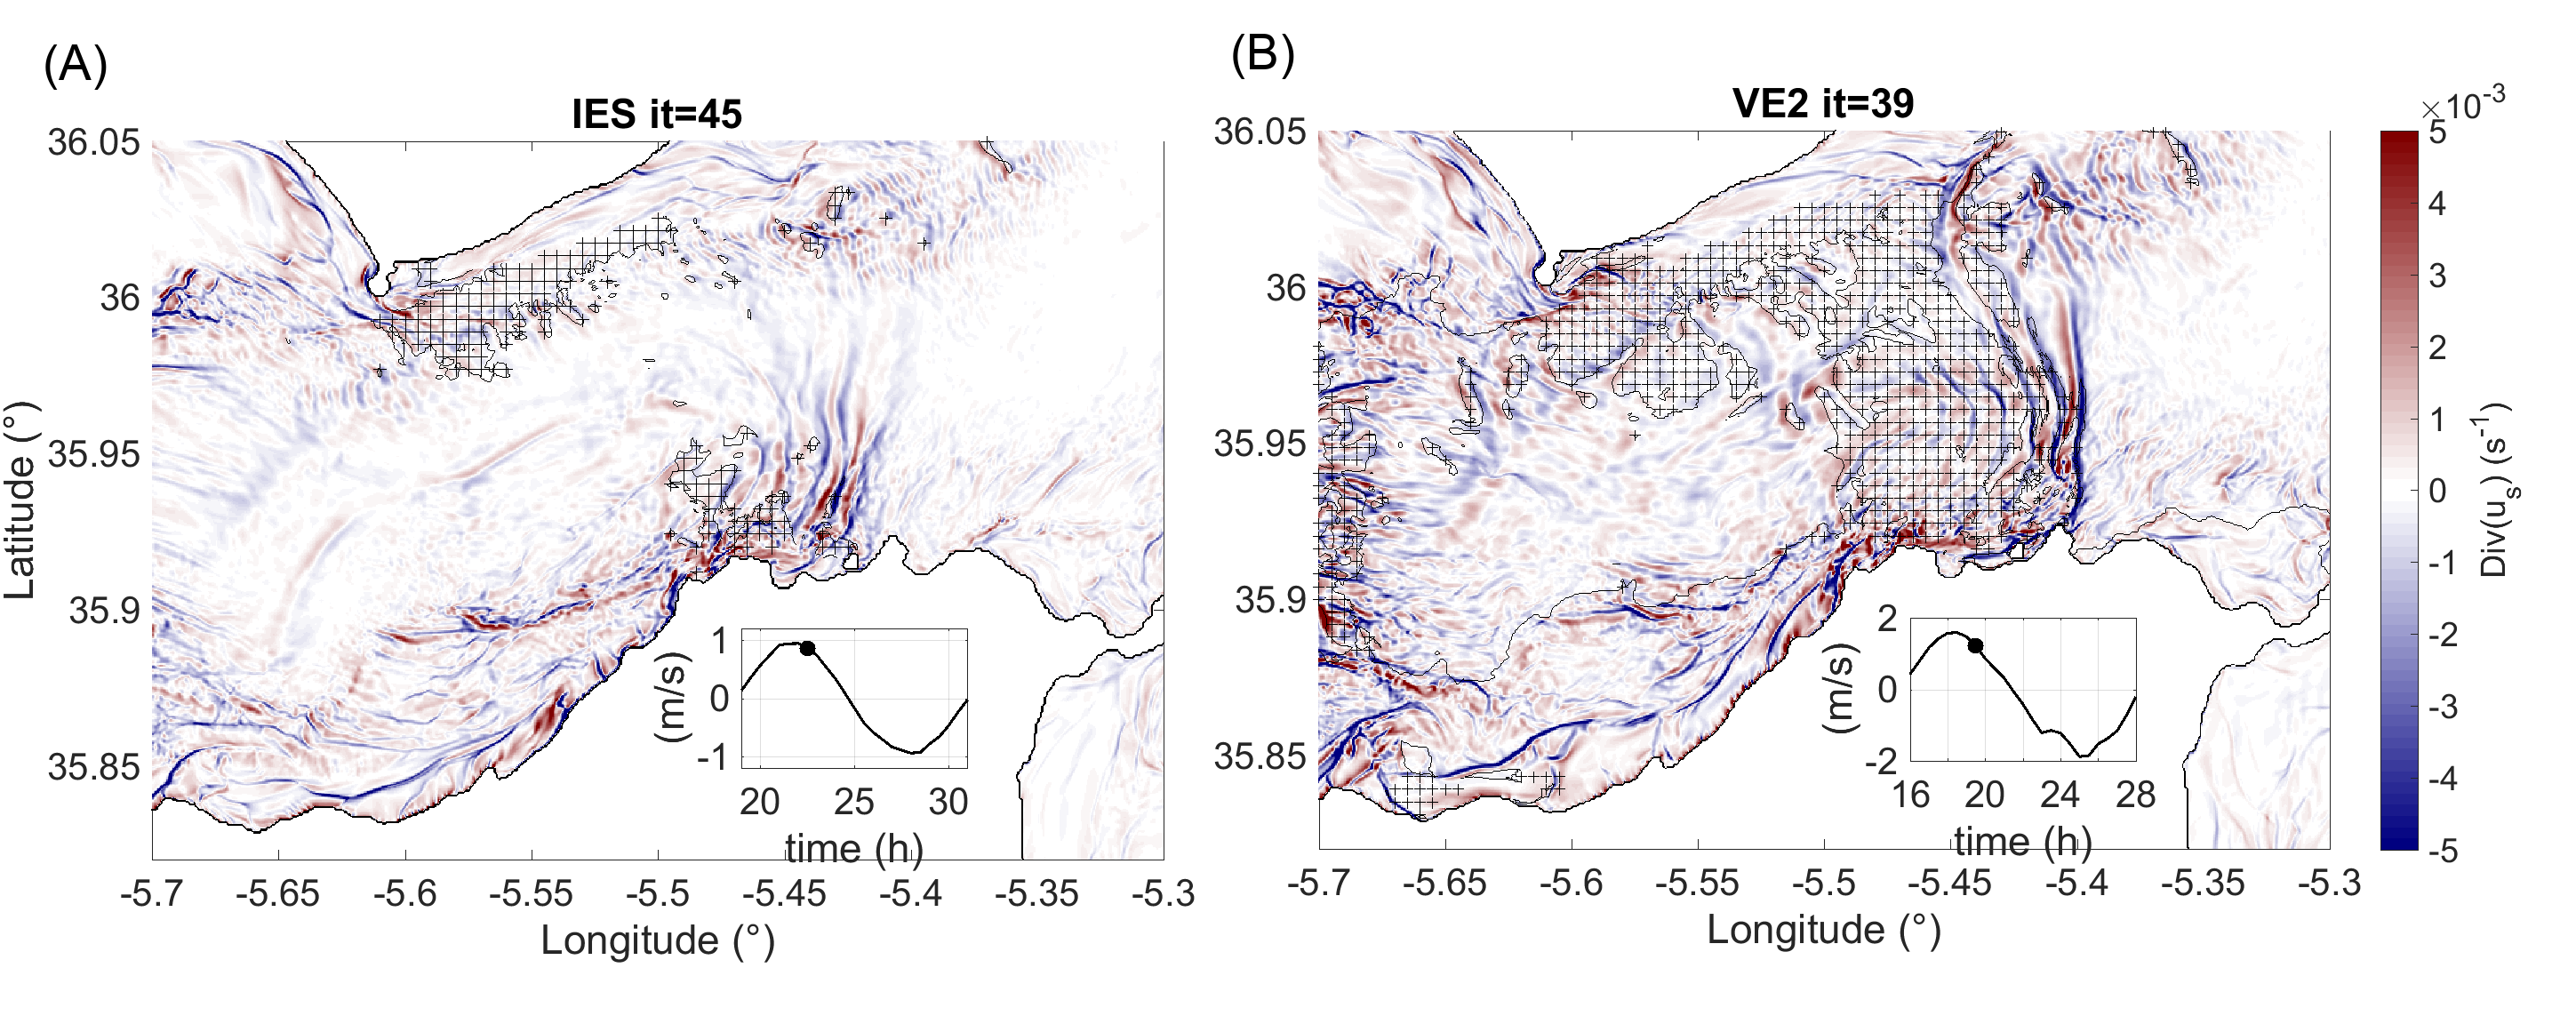
\includegraphics[width=\linewidth]{./GBR3D/FigWaveCont.png}
%\end{subfigure}
 \caption {Divergence of surface current (color) and area of supercritical atlantic layer (black hatchs) at t=22.5H in SimIT (a) and t=19.5H in SimST (b)}
 \label{FigISWGBR3D}
\end{figure}


\subsubsection{Propagation of Solitons (ISWs)}



\begin{figure}[!h]
 \centering
 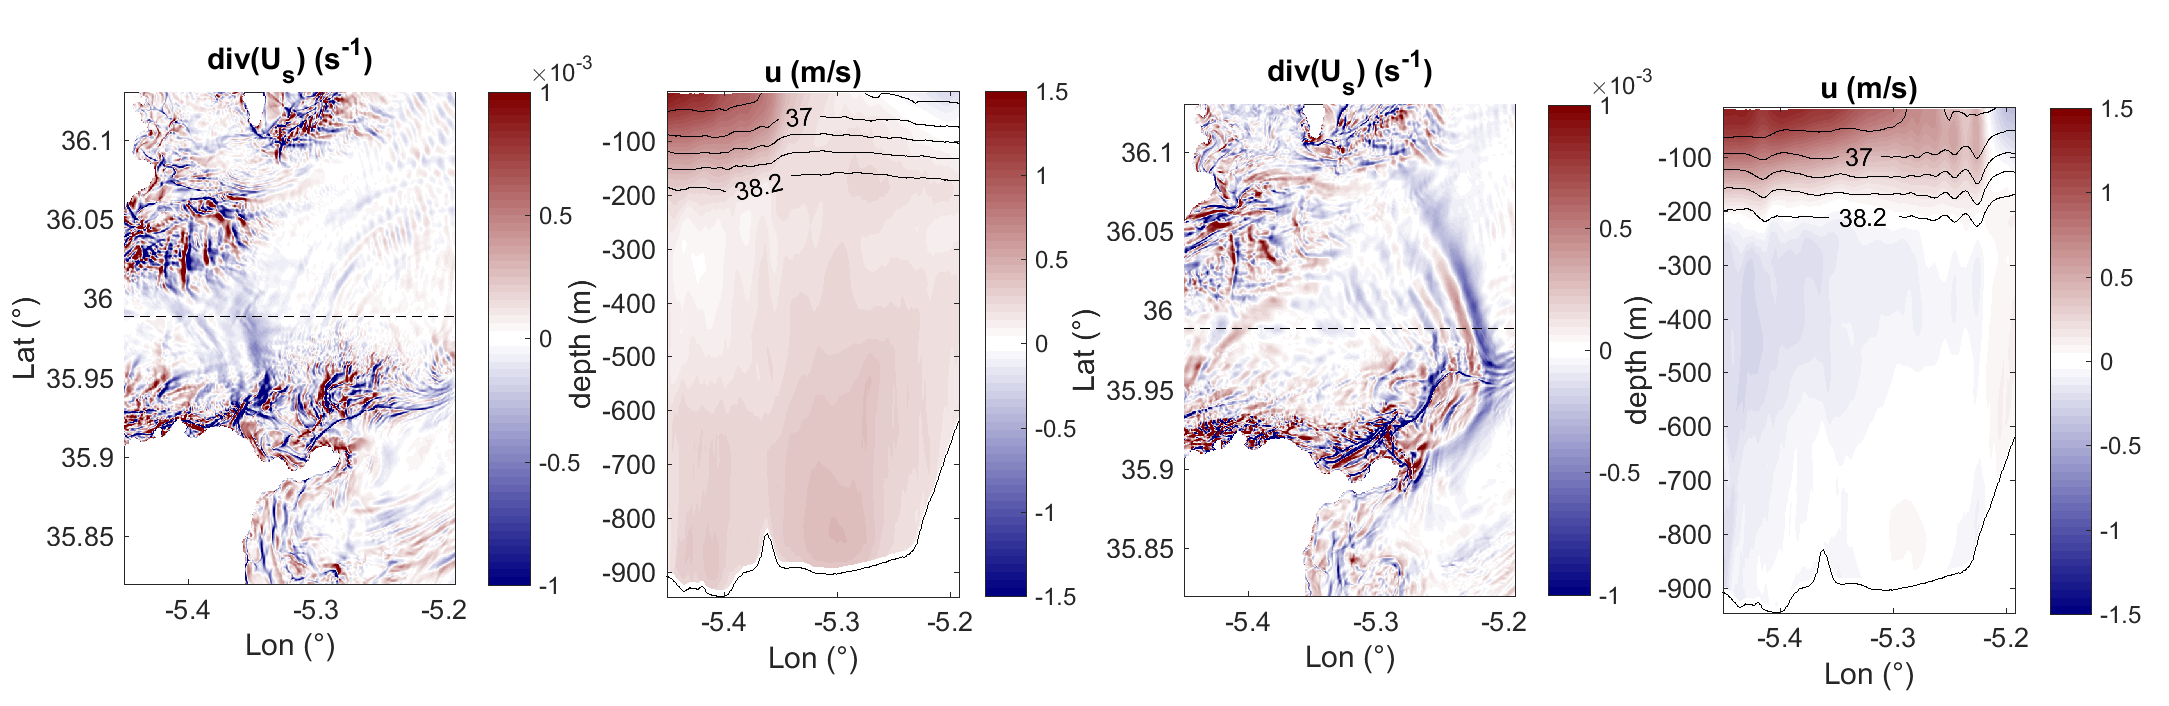
\includegraphics[width=1.\textwidth]{./GBR3D/coupesISW_ME2-2.png}
 \caption {Divergence of surface current (a,c) and vertical section (b,d) of salinity (black ishalines) and zonal velocity $u$ (color) in SimNT at 20h (a,b) and 22h (c,d) of simulation.}
  \label{FigISWNT}
\end{figure}



\begin{figure}[!h]
 \centering
%\begin{subfigure}{\linewidth}
%\centering
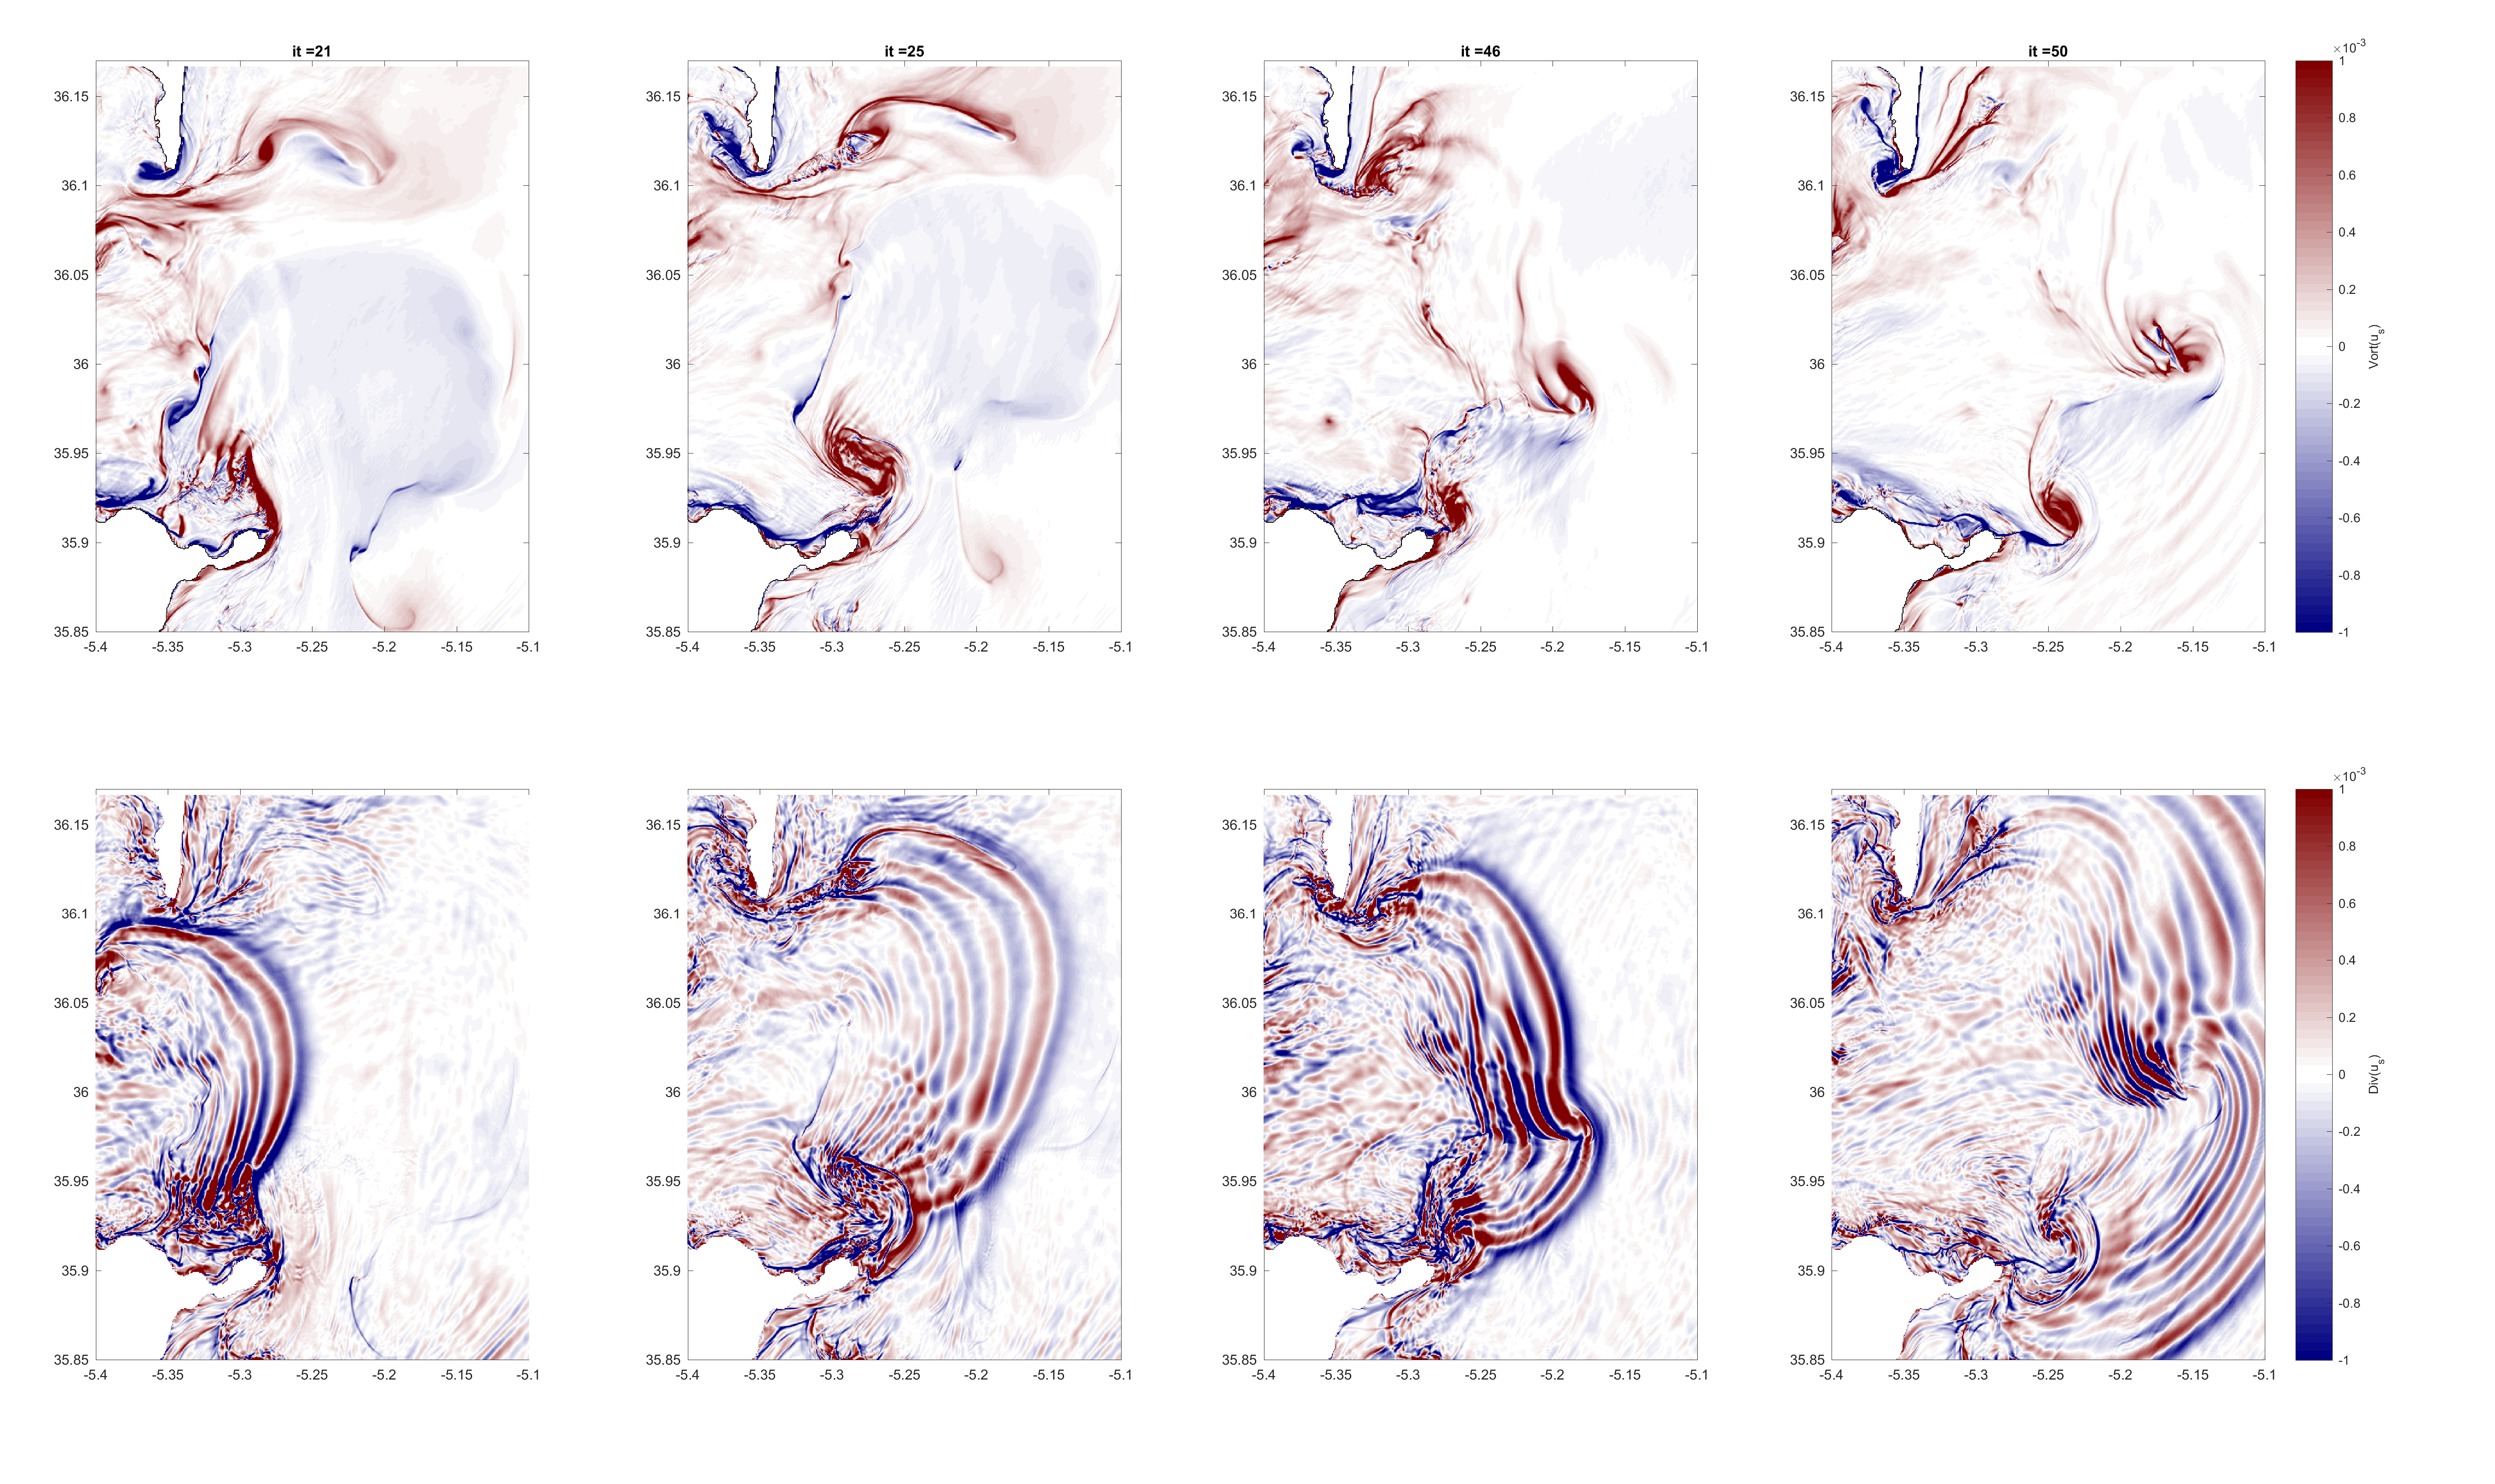
\includegraphics[width=\linewidth]{./GBR3D/FigTourbVE2.png}
%\end{subfigure}
 \caption {Divergence of surface current (upper row) at t=10.5H,12.5H, then 23H and 25H of simulation SimST,  and z-axis vorticity of surface current (lower row) for the same time.}
 \label{FigeddGBR3D}
\end{figure}

Solitary waves are observed as the relaxation of the hydraulic jump at CS as is the case in figure \ref{FigISWGBR3D}. Figure \ref{FigISWNT}.a and c also depicts the divergence of surface current but at the eastern exit of the Strait in inflow following a no-jump outflow. Figures \ref{FigISWNT}.b and d are vertical sections of zonal current and salinity at the same times. Can see that a train of solitary wave still ends up propagating in the alboran Sea, as the signal of the propagation of the baroclinic tide in figure \ref{FigISWNT}.b makes a more and more pronounced front with isohaline steepening due to non-linear effects. As is the case for the ISW generated at CS, non-hydrostatic dispersion balances this effect to create a train of solitary waves. In SimNT this process occurs following all \textit{no-jump} outflows.

However, compared to the upper row of figure \ref{FigeddGBR3D}, that also shows divergence of surface current but in tidal periods following hydraulic jump at CS, the train of solitary waves that are observed in Alboran Sea after a \textit{no-jump} outflow are less extended/have fewer waves. 

Figure \ref{FigeddGBR3D}.a,b then c,d show two inflows separated by one tidal cycle in simulation SimST. The lower row of figure shows the z-axis vorticity of surface currents at the same time. In the first two figures of each row, a train of solitary waves exits the Strait an enter Alboran Sea, the number of waves in the train increasing. A filament of positive vorticity is formed by interaction with the south coast in (e) and develops into a cyclonic eddy in (f). In \ref{FigeddGBR3D}.c one tidal cycle later the eddy is at 5.2$^\text{o}$W and 36$^\text{o}$N and the shape of the new train of solitary waves is refracted by this feature, south part accelerated and north part decelerated by the induced currents. At the same time can see once again vorticity patch off of Ceuta. In \ref{FigeddGBR3D}.d this patch too has developed in a cyclonic eddy that propagates in the Alboran Sea while the interaction between the solitary waves and the previous cyclonic eddy has resulted in an interference pattern in the wave packet. 


In the simulations, this process of generation of cyclonic eddy off of the coast of Ceuta occurs each time solitary waves exit the strait,  The wave of the next tidal cycle gets diffracted on this eddy, creating locally interference in the train of solitary waves.



\subsubsection{Dynamic at Camarinal Sill, primary instabilities}

\subparagraph{Neap-tide cycle}

Along with the features of the flow already discussed previously, figures \ref{FigHCN},\ref{FigHCS},and\ref{FigHCI} indicate patches of high standard deviation of parameter Q. They are the most extended for all outflow cases and for the spring tide inflow, although the values for this latter case are not as high and the patch is not as extended. High values of this parameter indicate oscillation of the value of parameter Q of greater amplitude, the highest are found for the two outflow case where hydraulic jump is detected (\textit{w-jump} and \textit{s-jump}), in the area west of CS at 5.79$^\text{o}$W and west of secondary bathymetric features in Tangier basin at 5.84$^\text{o}$W. There is also a lesser signal at Espartel Sill, of greater standard deviation for the spring tide outflow.

Figure \ref{FigTSCS}.a superposes to the standard deviation the singular vector of SVD performed on the 3D field of parameter Q computed during the outflow for the EOF that had the most high-frequency variability in its eigenvector, associated with propagation of vortices (the higher order EOFs (not shown) have low frequency variability and structure associated with the regional flow itself). As expected, the contour of parameter Q$=5e-5m^2s^{-2}$ in the EOF are located at same place as values of high standard deviation, on the west slope of Camainal Sill and the west slope of secondary sills in Tangier Bassin. 

Figures \ref{FigTSCS}.b to e show the partial view of $\theta$-S diagram of each gridpoint in the simulation at a given longitude, zoomed in on the part of the graph of med waters. See that in b that at 5.76$^text{o}$W, still over the crest of the sill, the repartition among mediterranean waters is still alike the one found in figure \ref{Fig_Ini_WM3D} at the east entry of the strait. Then from c to d, as look at more westward along the path of the mediterranean outflow, find the water parcels at close latitudes are homogenizing as three to four water masses.

These diagrams are plotted for longitudes close after the areas of high values of Q, where expected to have mixing processes, however not homogeneous water masses directly after CS. Look into it with 

\begin{figure}[!h]
% \centering
 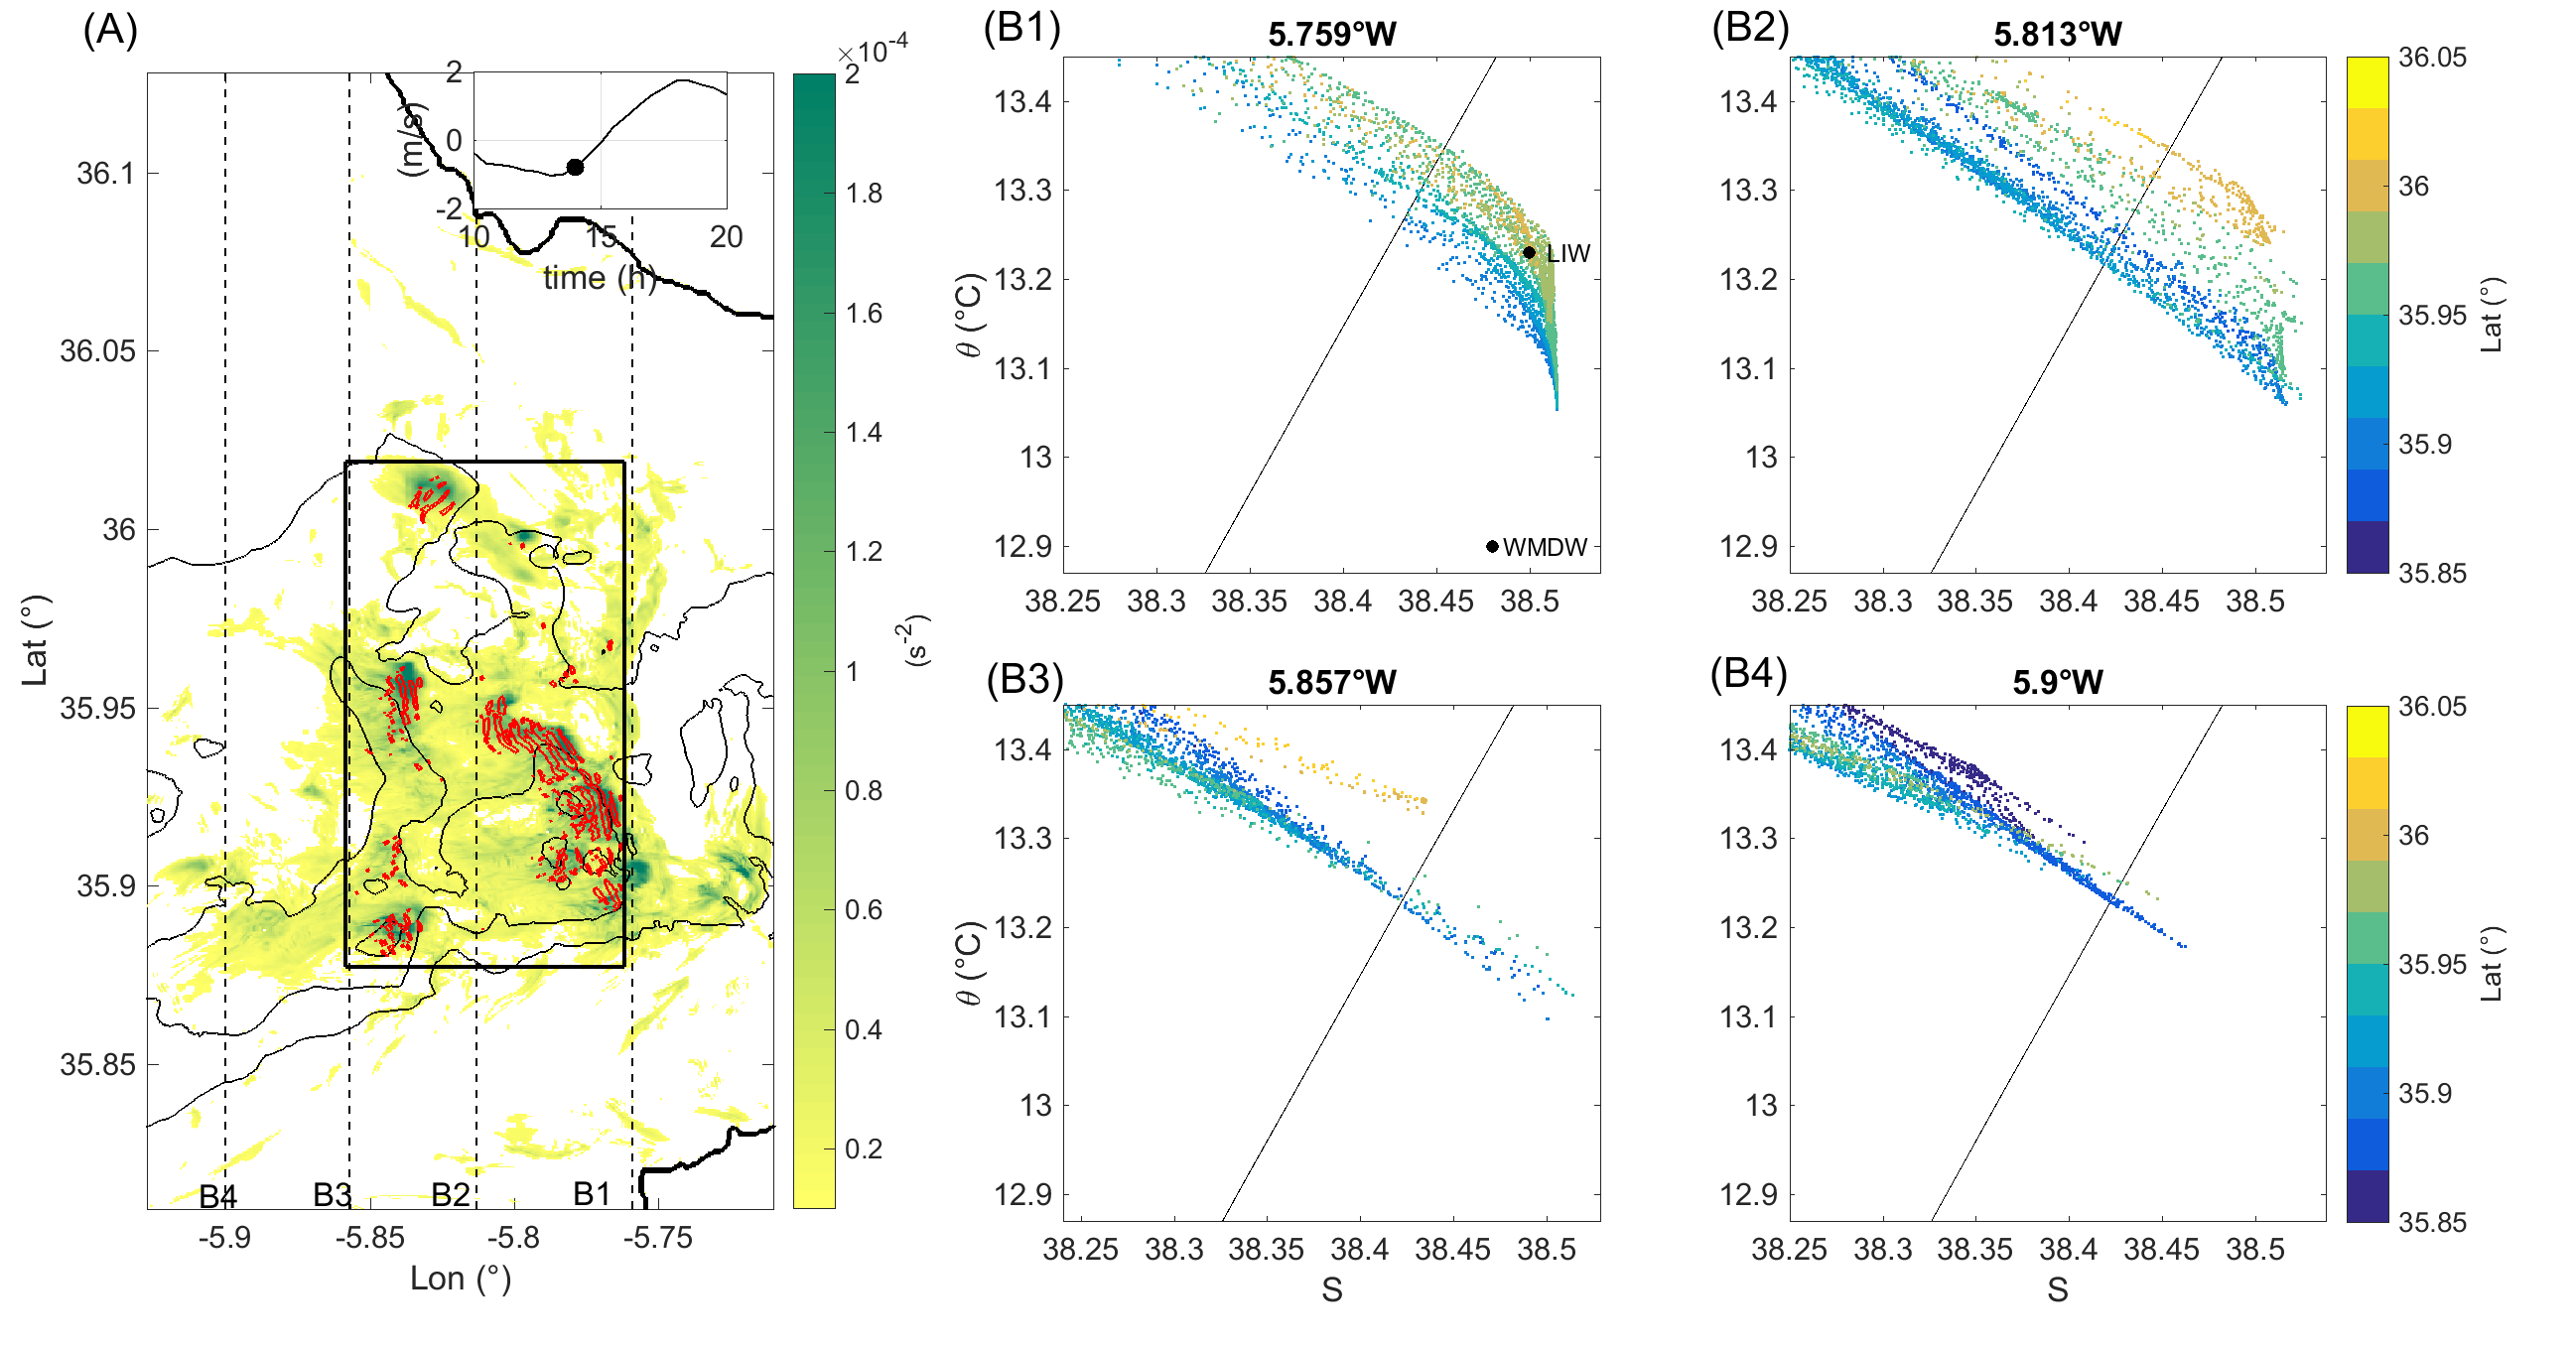
\includegraphics[width=\textwidth]{./GBR3D/TS_coupes_14H_VE2o.png}
 \caption {(a) Standard deviation of parameter Q over 30 mintues at t=14H in SimST (color) and trace of Q$=5$ from the high-frequency EOF of SVD performed in the rectangular black box during the outflow period. Black dashed lines indicate the longitude at which T,S diagrams are plotted. (b,c,d,e) T,S diagrams, zoomed in on area of Mediterranean watermasses. (Mettre LETTRES, rajouer section plus au sud?)}
 \label{FigTSCS}
\end{figure}


Now looking at the singular vectors of SVD for outflows of different strength of barotropic tidal currents . Figure \ref{FigEOFMIV}.a,b,c presents the EOF of parameter Q for the outflows of figures \ref{FigHCN},\ref{FigHCS},and\ref{FigHCI},along with vertical sections of salinity at the time of figure \ref{FigEOFMIV}d,e,f plotted along latitude 35.94$^\text{o}$N. Figure \ref{FigEOFMIV} g and h are histograms giving the height above seafloor and latitude of the grid points of the EOF for which Q$\geq 5e-5m^2/s^2$. On vertical sections, can see that the positive value of Q parameter are associated with billow structures of salinity that develop in the gravity current along the west slope of the Camarinal Sill. Those structures develop for each outflow case, but the wider distributions of height above sea floor and visualisation in the vertical section indicates the billows have greater radius in the hydraulic jumps cases, entraining more interfacial and atlantic waters into the mediterranean outflow. At this longitude where the instabilities are still developed, cores are not yet mixed in the simulation, can see as in the $\Theta$-S diagrams that the outflow is still heterogeneous.

The two hydraulic jump cases also differ, while instabilities develop along the same areas in no-jump and s-jump case, in the w-jump case the hydraulic jump and the start of the gravity current are co-localised at all latitude as seen in the vertical section, which adds a possible area of generation between 35.92$^\text{o}$N and 35.93$^\text{o}$N, down slope of the shallowest point of the sill where the flow of Mediterranean waters is not as strong for s-jump and no-jump cases.


\begin{figure}[!h]
% \centering
 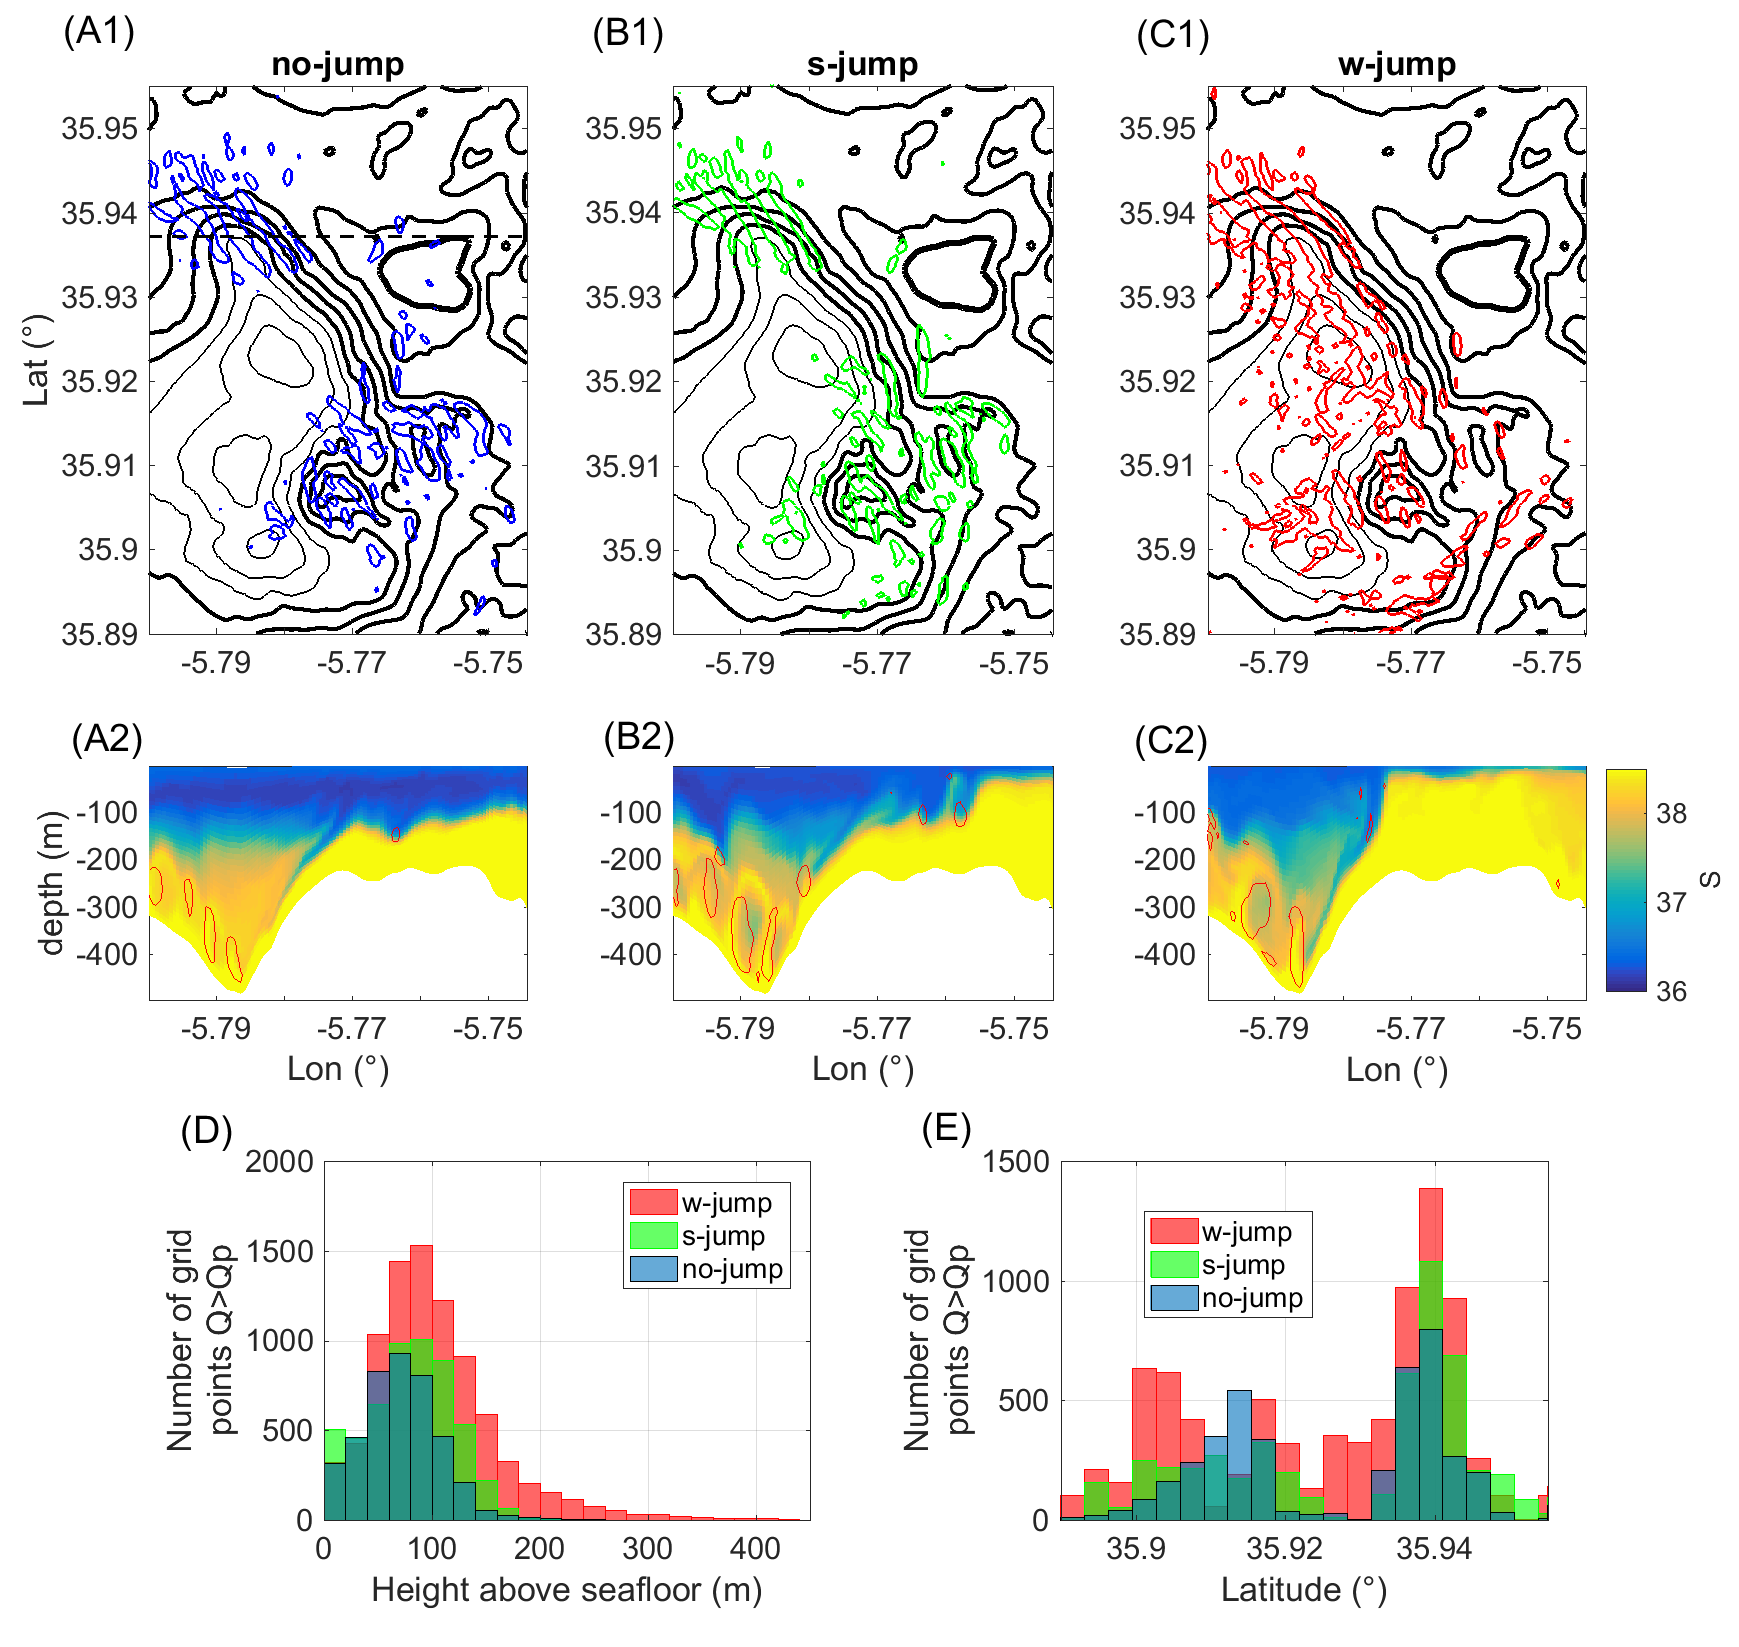
\includegraphics[width=\textwidth]{./GBR3D/EOF5_MIV_2D.png}
 \caption {(a,b,c) Contour of parameter Q$=5.10^{-5}$ in first high frequency EOF of SVD performed during outflow of figures \ref{FigHCN}.b,\ref{FigHCI} and \ref{FigHCS}.b respectively. and isobathes (black) (200m, thicker)  (250 to 450, thick) (500 to 600m, thin). (d,e,f) vertical section of salinity (color) and contour of Q-parameter $=5.10^{-5}$ at latitude $35.9372^\text{o}$ at the same time as figures \ref{FigHCN}.b,\ref{FigHCI} and \ref{FigHCS}.b respectively. (g) histogram of the height of the grid points of each EOF shown in a,b and c above the seafloor. (h) histogram of the latitude of the grid points of each EOF shown in a,b and c above the seafloar. }
 \label{FigEOFMIV}
\end{figure}


\subparagraph{Closure scheme}

Now look at four other simulations, three use Smagorinsky turbulent scheme with different coefficients. One is using GLS K-$\epsilon$. In figure \ref{Fig3Dsch}.a,c,e,g, vertical section of salinity during the first outflow at t$=$5h of simulation which is in a no-jump case, with Richardson gradient number $Ri$ and Q parameter indicated. $Ri$ is calculated from fields of density and velocity averaged over a half hour to filter out the propagating structures.

Figure \ref{Fig3Dsch}.b,d,f,h the averaged salinity in med (b,f) and atl layer(d,h),east (f,h) and west (b,d) of Camarinal Sill. Note that this is averaged value, as shown in figure \ref{FigTSCS} and can be seen in the vertical sections the outflow/med layer is not homogeneous at this longitude yet/those longitudes.


Looking at averaged layer salinities east of the Sill in figures \ref{Fig3Dsch} f,h, see that simulations SimIT-S001, SimIT-S01 and SimIT-Kep have same salinities for med layer, and can see some differences in atl layer punctually. , the simulations most different is SimIT-S1 that has a less salty med layer and a saltier atl layer. This is logical as with the enhanced mixing coefficient, more diffusion in the pycnocline between the two layers.

However, while the atl layer is again saltier west of the sill for SimIT-S1, so is the mediterranean layer, especially between 2 and 8 houyrs of simulation, which shouldn't be the case if only diffusion. Looking at the vertical section at 5 hours of simulation can see that instabilities develop for all of them. However, while can see that the area of $Ri=0.25$ starts at 5.77$^\text{o}$ for all four simulations, indicating shear instabilities could develop from this point in the gravity current, for simulation SimIT-S1 they start down slope of an intrusion of atlantic waters at 5.783$^\text{o}$W. While the other simulations, the salinity entrained by teh billows is from the altantic layer//contain less salty waters, ie the signal of atl surface water in the med outflow will be stronger in this simulation.

More atl waters incorporated for Kepsilon, for which the billows are not as developped, instabilitied less developed with smaller values of parameter Q (closer to a gravity current only?), and less salty outflow. This signal persists after $t=7h$ when the flow reverses and no more generation of instabilities, and in a lesser extent for SimIT-S1 for which the effect of more diffusion in the pycnocline may counteract with the injected med water.


While the width of the Med vein as it begins to go down slope of Camarinal as salty water is the same, in simulations 1 and 2 instabilities are earlier in the jump and bring more atl waters as the core or billows are advected down slope, resulting in more atl water being integrated to the med outflow at the passage of CS. 






\begin{figure}[!h]
% \centering
 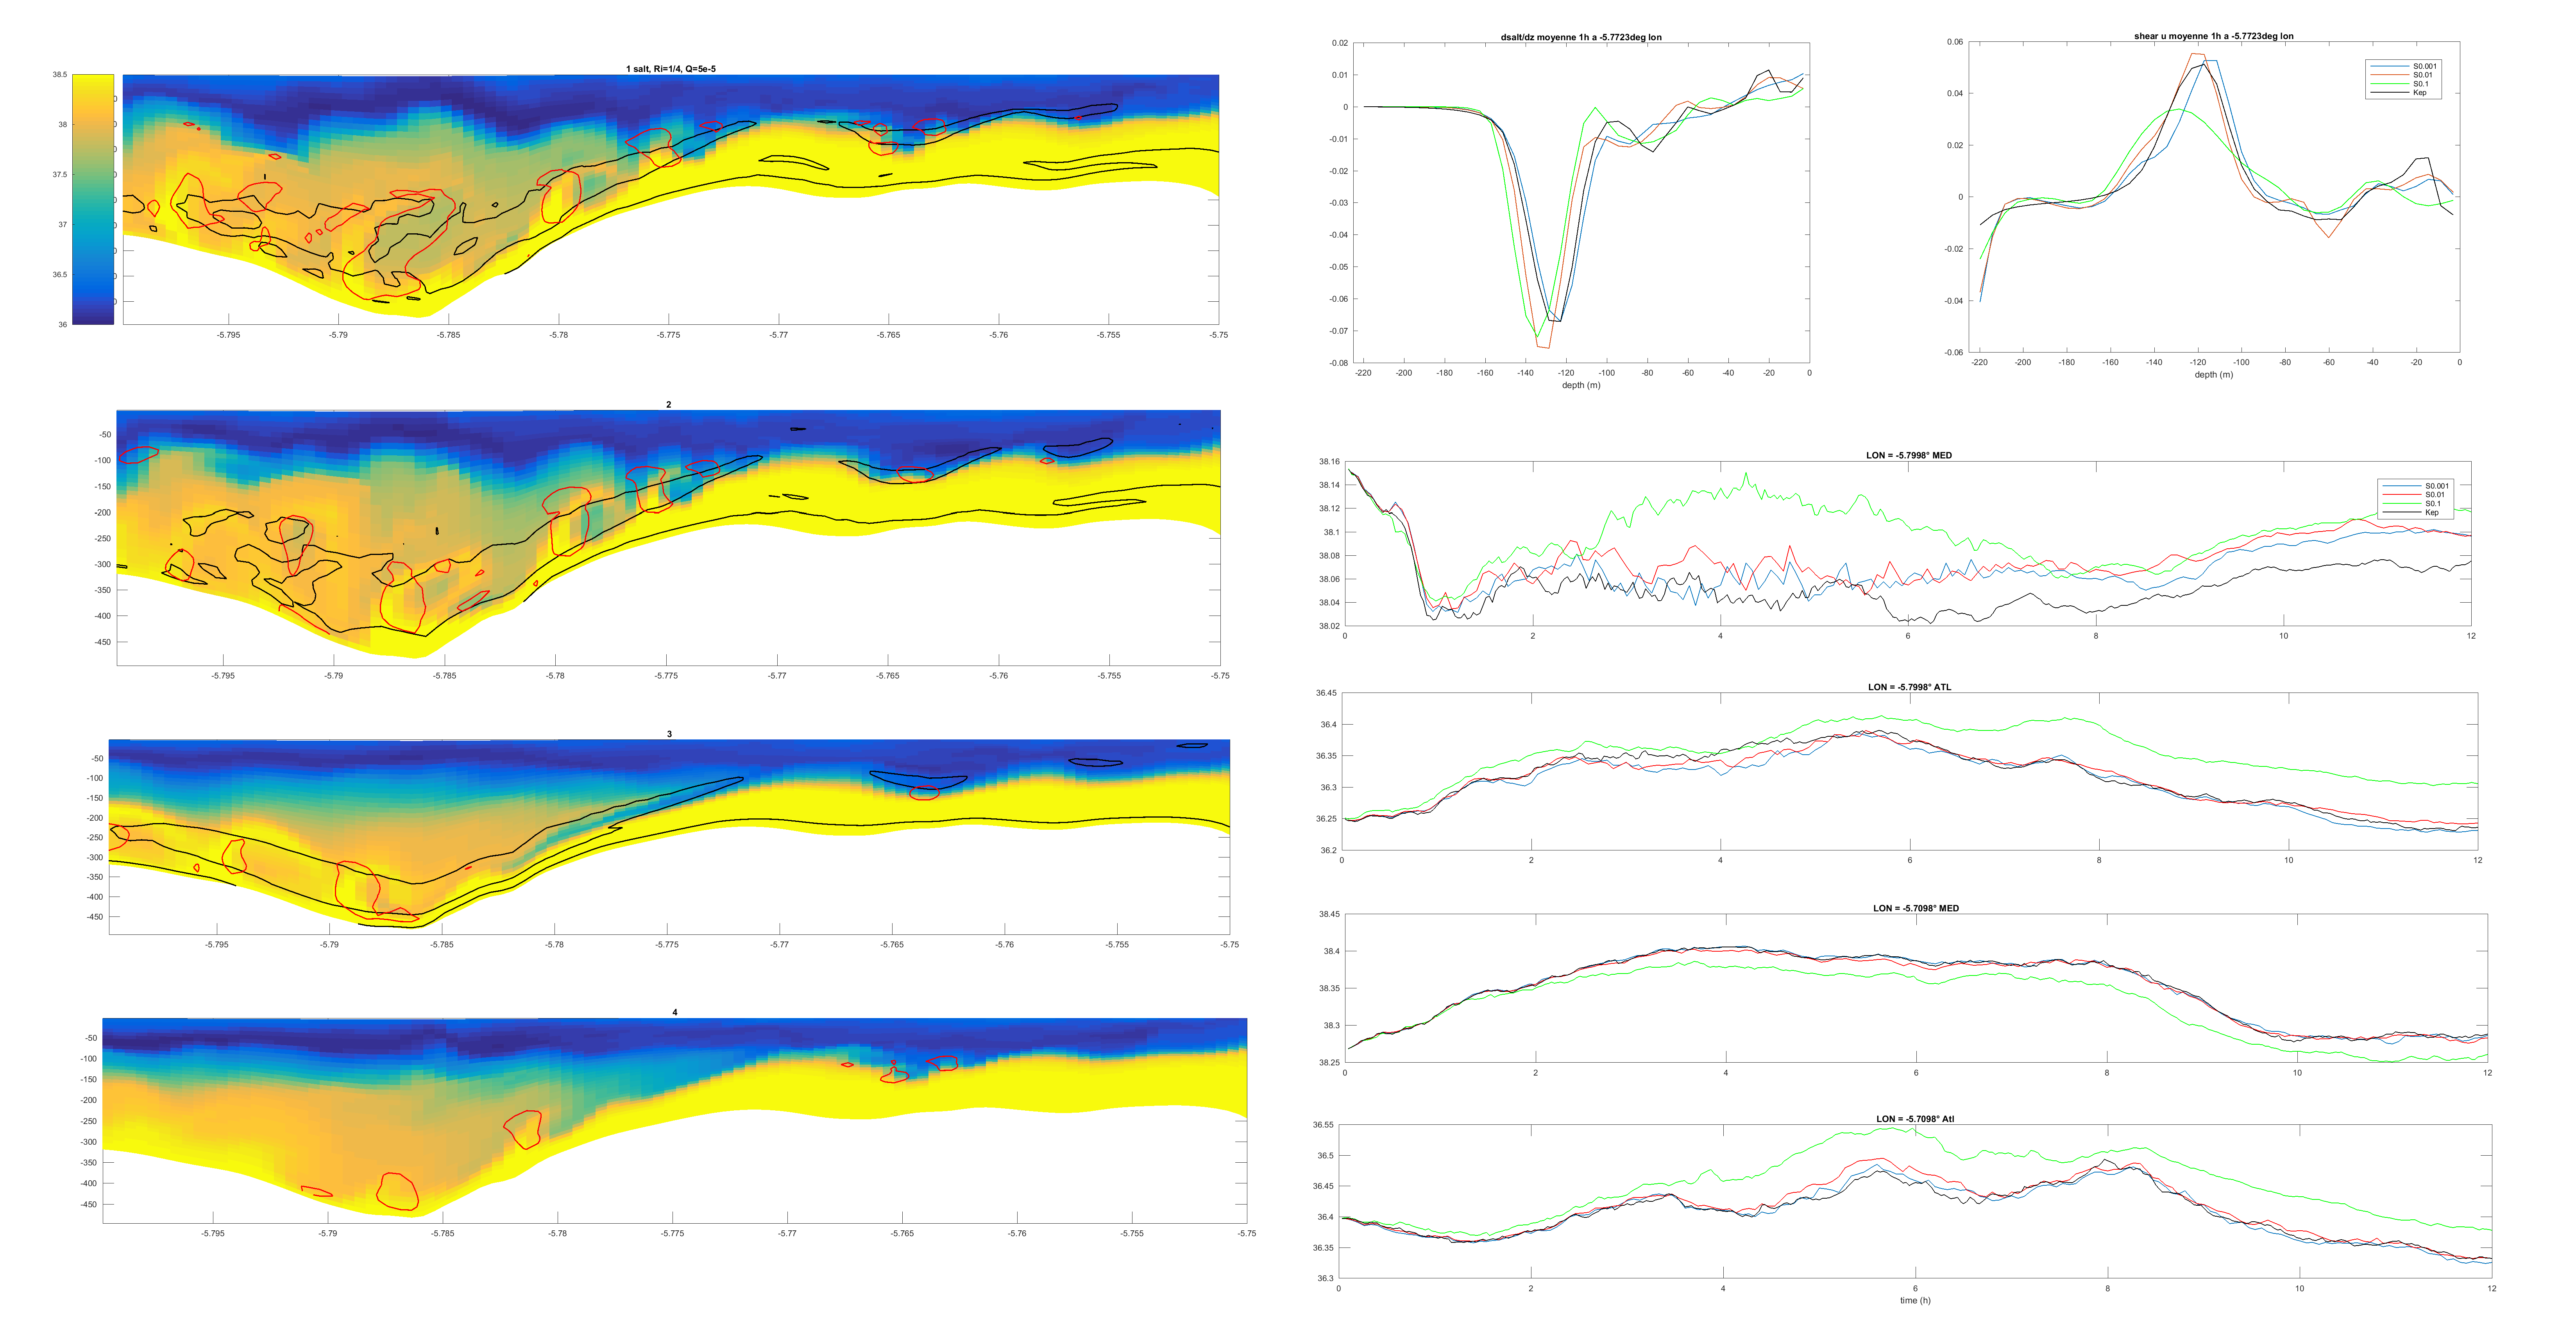
\includegraphics[width=\textwidth]{./GBR3D/Figsmago.png}
 \caption {Vertical section of salinity (color) and contour of $Q=5.10^{-5}$ (red) and Richardson gradient number $=025$ (black) at lat = $35.9372^o$ in simulations SimIT-S001,SimIT-S01,SimIT-S1 and SimIT-Kep IES at t=4h of simulation. time  (1:S0.001  2:S0.01  3:S0.1 4:Kep)(Rajouter une évolution de ubar!!! sur s0.001)}
 \label{Fig3Dsch}
\end{figure}

%-------------------------------------------------------------------------------------
\subsection{Conclusion}

Have looked into the variability in neap-spring tidal cycle of hydraulic control and other features in high resolution non hydrostatic simulation of the strait of Gibraltar.See no permanent supercritical flow across the simulations, only intermittent with the tidal cycle, with location and extension of the area of supercritical flow depending on the strength of the barotropic currents.

In outflow when both atl and med layers are critical, hydraulic jump, which position is either over the shallowest part of the sill, or over its western slope. This hydraulic jump evolves into train of solitary waves, as expected once hydraulic control is lost near high tide, that exits the strait into the Alboran Sea. Even for tidal cycle for which the flow over the sill is not critical and there is no formation of hydraulic jump, the non-linearity of the propagation of the barotropic tidal signal in the eastern part of the strait devolves into a less extended train of solitary waves propagating into the Alboran Sea.At each simulated tidal cycle, a cyclonic eddy is formed of the coast of Ceuta in the southern part of the eastern exit of the Strait. This eddy is advected by the flow in th Alboran Sea and interacts with the train of solitary waves, locally diffracting the waves.


Other feature present in simulations are the billows/shear instabilities developing in the lee of CS. In simulations, these billows are associated with high positive values of parameter Q that is used as proxy for their detection and analysis. The billows are generated at interface of med and atl waters and advected by the med outflow.   they are also present at secondary relief in tangier basin and at espartel sill. They are present during outflows of all intensity, but their repartition will change with intensity of tidal currents. They have a role in the way the med water is mixed, with changes of hydrological features of the med vein, and in simulation the way this mixing occurs is sensible to the dynamic of the instabilities that is piloted by the turbulent dissipation scheme.


 Can see that the configuration of the flow at CS, by being the first passage of the Med waters, will affect the hydrological properties of the Mediterranean outflow, first by the volume of med waters that can flow west of the sill at each outflow, second by how much Atlantic waters are being mixed into it.

However, it is important to note that simulation only represents the beginning of the mixing by turbulent processes, in particular, no secondary evolution of KH instabilities.


Moreover, The lack of atmospheric forcing probably means inaccuracies of features of the upper layer, especially circulation of the Atlantic layer in Tarifa Narrows where wind stress affects the upper layer. This could explain why have the baroclinic tide degenerate into an internal bore then a train of solitary waves for all inflows following a \textit{no-jump} outflow at CS, whereas observations indicate that in neap tide do not have solitary waves at each tidal cycle. Other processes could be affected like the formation of eddy at the exit of the Strait that occurs at the coast and its advection into Alboran that is probably influenced by the WAG.
